\documentclass[a4paper, 12pt]{extarticle}

% Includes 
\usepackage[utf8]{inputenc} % UTF-8 encode 
\usepackage[english, russian]{babel}
\usepackage{geometry} % adjust page layout 
\usepackage{graphicx} 
\usepackage{hyperref} 
\usepackage{amsmath} % math formulas 
\usepackage{setspace} % for set line spacing 
\usepackage{indentfirst} % indent on a first line after the paragraph 
% \usepackage{pgfplots} % for plots 
\usepackage{listings} % for code listings 
\usepackage{xcolor} % colors (used for listings)
\usepackage{sourcecodepro} % for another monospaced font 
\usepackage{cmap} % for correct search in pdf
\usepackage{placeins} % for floatbarrier


% debug
% \usepackage{showframe} % frame borders for demonstration 

%%% Custom commands
% commands for unnumbered sections
\newcommand{\usection}[1]{\section*{#1} \addcontentsline{toc}{section}{\protect\numberline{}#1}}
\newcommand{\usubsection}[1]{\subsection*{#1} \addcontentsline{toc}{subsection}{\protect\numberline{}#1}}
\newcommand{\usubsubsection}[1]{\subsubsection*{#1} \addcontentsline{toc}{subsubsection}{\protect\numberline{}#1}}

\DeclareMathOperator{\sinc}{sinc}

% Redefinition of section and subsection numbering style
\def\thesection{\arabic{section}.}
\def\thesubsection{\arabic{section}.\arabic{subsection}.}
\def\thesubsubsection{\arabic{section}.\arabic{subsection}.\arabic{subsubsection}.}



% Settings for links 
\hypersetup{
    colorlinks,
    citecolor=black,
    filecolor=black,
    linkcolor=black,
    urlcolor=black
}


% Layout
\geometry{
	left=17mm,
	top=17mm,
	right=17mm,
	bottom=20mm,
	marginparsep=0mm,
	marginparwidth=0mm,
	headheight=8mm,
	headsep=5mm, 
}

\linespread{1.5} % line spacing
\setlength{\parskip}{\baselineskip}  % Add space between paragraphs


% overfull hbox settings
\tolerance 10000 % default 200, max 10000
\hbadness 10000 % default 1000, max 10000
\emergencystretch 0pt  % default 0pt, how much the lines can stretch for the sake of good line breaks
\hfuzz 0.4pt % ignore overfull box less than 
\widowpenalty=10000 % no lines at the start of the page
\vfuzz \hfuzz % don't care about underfull vbox if overfull is acceptable
\raggedbottom % if the page is not filled, align the content to the bottom


% Redefinition of table of contents command to get centered heading
\makeatletter
\renewcommand\tableofcontents{ 
  \begin{singlespace}
    \null\hfill\textbf{\Large\contentsname}\hfill\null\par
    \@mkboth{\MakeUppercase\contentsname}{\MakeUppercase\contentsname}%
    \@starttoc{toc}
  \end{singlespace}
}
\makeatother


% Listings settings
\definecolor{codegreen}{rgb}{0, 0.6, 0}
\definecolor{codegray}{rgb}{0.5, 0.5, 0.5}
\definecolor{codepurple}{rgb}{0.58, 0, 0.82}
\definecolor{backcolour_gray}{rgb}{0.98, 0.98, 0.98}

\lstdefinestyle{python_white}{
  language=Python,
  backgroundcolor=\color{backcolour_gray},   
  commentstyle=\color{codegreen},
  keywordstyle=\color{blue},
  numberstyle=\tiny\color{codegray},
  stringstyle=\color{codepurple},
  basicstyle=\ttfamily\small\singlespacing,
  breakatwhitespace=true,         
  breaklines=true,                 
  captionpos=b, % t/b                  
  keepspaces=true,                 
  numbers=none, % none/left/rigth                    
  numbersep=5pt,                  
  showspaces=false,                
  showstringspaces=false,
  showtabs=false,                  
  tabsize=2,
  frame=single, % none/leftline/topline/bottomline/lines/single/shadowbox
  rulecolor=\color{gray}, % frame color 
}


\lstset{style=python_white}


% For title page
\def\name{Отчет по лабораторной работе №2} 
\def\subname{Преобразования Фурье}
\def\madeby{Александр Иванов, R3238, ЧМ 1.2}
\def\teacher{Перегудин А. А.}

\begin{document}

% Title page 
\begin{titlepage}

\thispagestyle{empty}

\title{


\includegraphics[width=4cm]{media/ITMO_logo.png} 

\vspace{1em}
НИУ ИТМО 
\vspace{4em}

\begin{center}
\large\textsc{\textbf{\name}}

\vspace{1em}
``\subname'' 

\end{center}

\vspace{3em}

\begin{flushright}
\normalsize{ 
Выполнил: \\ \textbf{\madeby} 

Преподаватель: \\ \textbf{\teacher} 
}
\end{flushright}	

\vfill

\begin{center}
\small{Санкт-Петербург, \the\year}
\end{center}
}


\author{}
\date{}
\maketitle
\thispagestyle{empty}
\end{titlepage} % Title page

\addtocounter{page}{1} % Inc counter to start from 2 
\tableofcontents % Table of contents
\pagebreak

\section{Спектральное дифференцирование}

\subsection{Исходная функция}
Рассмотрим функцию $f(t) = sin(t)$ и соответствующий ей массив точек на промежутке $[-10, 10]$ с 
наложенным на нее небольшой случайный шум. График полученный функции приведен на рисунке \ref{fig:noised_sin}.

\begin{figure}[ht!]
    \centering
    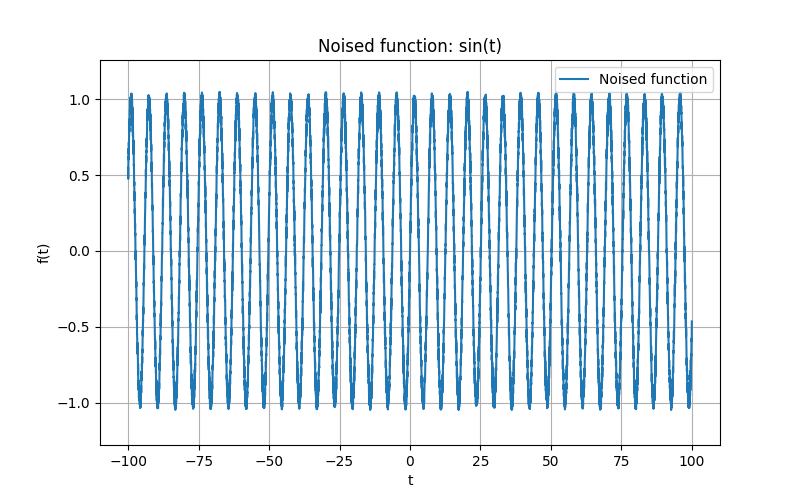
\includegraphics[width=\textwidth]{../results/10/noised_sin.png}
    \caption{Функция $f(t) = sin(t)$ с небольшим случайным шумом}
    \label{fig:noised_sin}
\end{figure}

\FloatBarrier
\subsection{Численная производная}
Найдем численную производную от зашумленной функции, используя поточечное дифференцирование: 
\begin{equation}
    f'(t) = \frac{y(k + 1) -  y(k)}{dt}
\end{equation}
график полученной производной приведен на рисунке \ref{fig:diff_noised_sin}.
На графике видно, что производная функции $f(t) = sin(t)$ с небольшим шумом также сильно зашумлена,
это связано, с тем, что значения исходной функции терпят сильные изменения за короткие промежутки времени.

\begin{figure}[ht!]
    \centering
    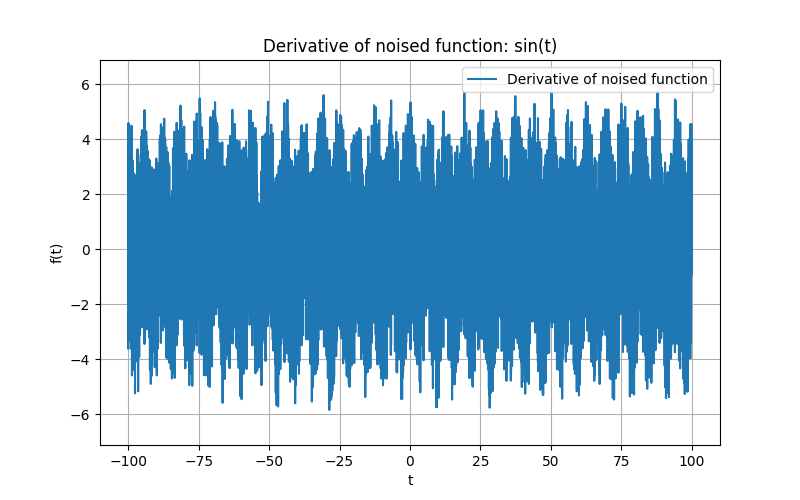
\includegraphics[width=\textwidth]{../results/10/noised_sin_derivative.png}
    \caption{Численная производная функции $f(t) = sin(t)$}
    \label{fig:diff_noised_sin}
\end{figure}

\FloatBarrier
\subsection{Спектральная производная}
Для нахождения спектральной производной найдем образ исходной функции $f(t)$ (см. рисунок \ref{fig:noised_sin_image}). 
\begin{figure}[ht!]
    \centering
    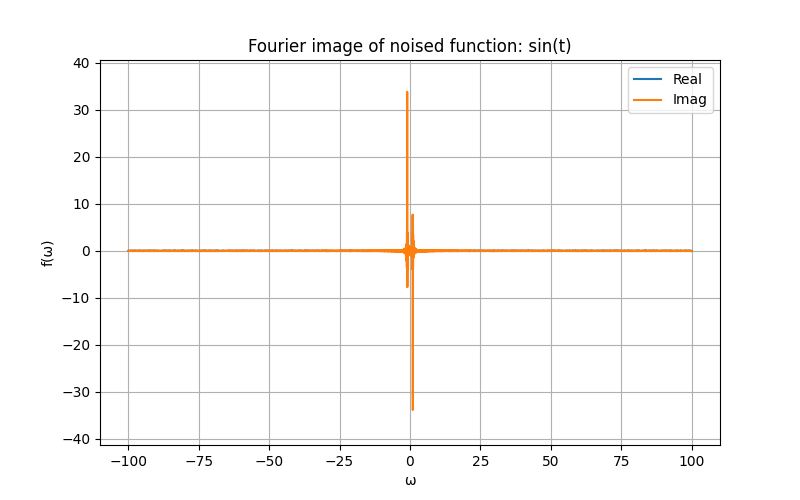
\includegraphics[width=\textwidth]{../results/10/noised_sin_image.png}
    \caption{Образ функции $f(t) = sin(t)$}
    \label{fig:noised_sin_image}
\end{figure}
Теперь, воспользовавшись тем, что:
\begin{equation}
    \mathcal{F}\{f'(t)\} = i \omega \mathcal{F}\{f(t)\}
\end{equation}
домножим образ функции на $i \omega$ и найдем обратное преобразование Фурье (см. рисунок \ref{fig:noised_sin_image_deriviate}).

\begin{figure}[ht!]
    \centering
    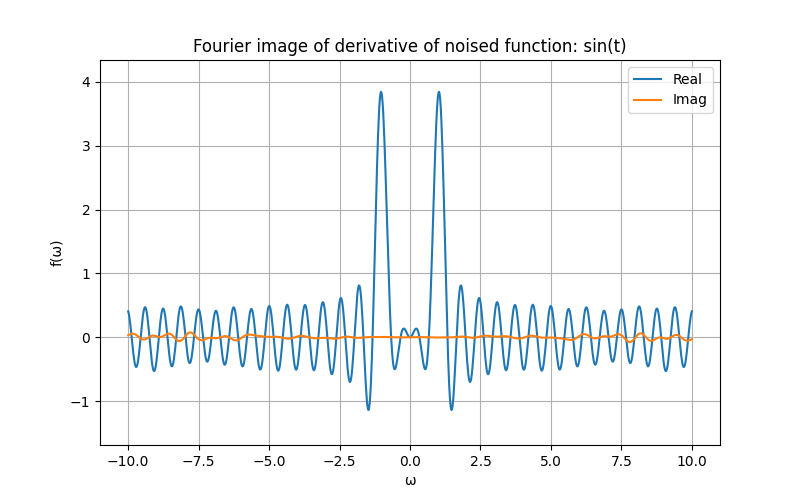
\includegraphics[width=\textwidth]{../results/10/noised_sin_image_derivative.png}
    \caption{Образ производной функции $f(t) = sin(t)$}
    \label{fig:noised_sin_image_deriviate}
\end{figure}
Найдем обратное преобразование Фурье от образа производной функции (см. рисунок \ref{fig:noised_sin_image_deriviate_restored}) и сравним его с численной производной и истиной производной $(cos(t))$ (см. рисунок \ref{fig:derivative_cmp}).

\begin{figure}[ht!]
    \centering
    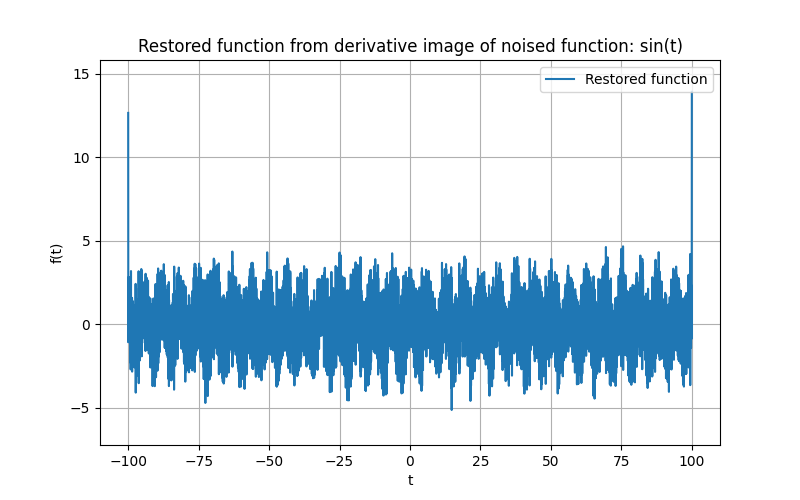
\includegraphics[width=\textwidth]{../results/10/noised_sin_image_derivative_restored.png}
    \caption{Обратное преобразование Фурье от образа производной функции $f(t) = sin(t)$}
    \label{fig:noised_sin_image_deriviate_restored}
\end{figure}

\begin{figure}[ht!]
    \centering
    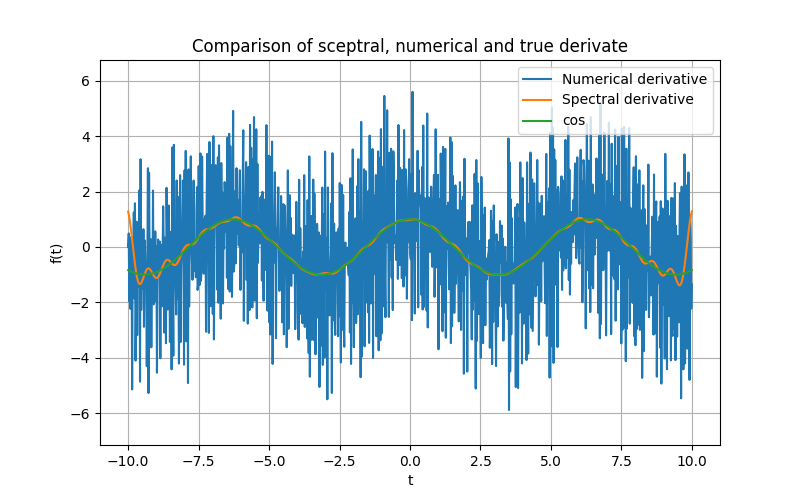
\includegraphics[width=\textwidth]{../results/10/derivative_cmp.png}
    \caption{Сравнение численной производной, истинной производной и спектральной производной}
    \label{fig:derivative_cmp}
\end{figure}

\FloatBarrier
На сравнительном графике (см. рисунок \ref{fig:derivative_cmp}) видно, что спектральная производная практически совпадает с истинной производной функции $f(t) = sin(t)$, в то время как численная производная сильно зашумлена и не совпадает с истинной.
Это, в первую очередь связано с тем, что при образ исходной функции $f(t)$ находился на промежутке $[-10, 10]$, а не на всей числовой прямой, что привело к фильтрации шума и улучшению качества производной. 

Графики для промежутка $[-100, 100]$ приведены в приложении \ref{app:A}, так как я посчитал их менее информативными и понятными. 

\FloatBarrier
\section{Линейные фильтры}

Для выполнения задания рассмотрим функцию $g(t)$, которая задается следующим образом: 
\begin{equation}
    g(t) = \begin{cases}
        a, & t \in [t_1, t_2]\\
        0, & otherwise
    \end{cases}
\end{equation}

Кроме того, зададим \textit{зашумленную} версию функции $u(t)$ 
\begin{equation}
    u(t) = g(t) + b(\rand(t) - 0.5) + c(\sin(d \cdot t))  
    \label{eq:noise}
\end{equation}


\subsection{Линейный фильтр первого порядка}

Будем рассматривать линейный фильтр первого порядка, который описывается следующим уравнением:
\begin{equation}
    W_1(p) = \frac{1}{Tp + 1}
\end{equation}
где $T$ -- постоянная времени.

\def\num{1}
\def\a{4}
\def\from{1}
\def\to{4}
\def\b{1}
\def\c{0}
\def\d{0}
\def\L{10}
\def\T{0.5}

\subsubsection{Рассматриваемая функция}
Рассмотрим функцию $g(t)$ при параметрах $a=\a$, $t_1 = \from$, $t_2 = \to$ ~(см. рисунок~\ref{fig:wave_func_\num}) 
и ее \textit{зашумленную} версию $u(t)$ с параметрами $b = \b$, $c = \c$, $d = \d$ ~(см. рисунок~\ref{fig:noised_wave_func_\num}).
на промежутке $[0,\L]$. 

\subsubsection{Графики рассматриваемой и зашумленной функции}
\begin{figure}[ht!]
    \centering
    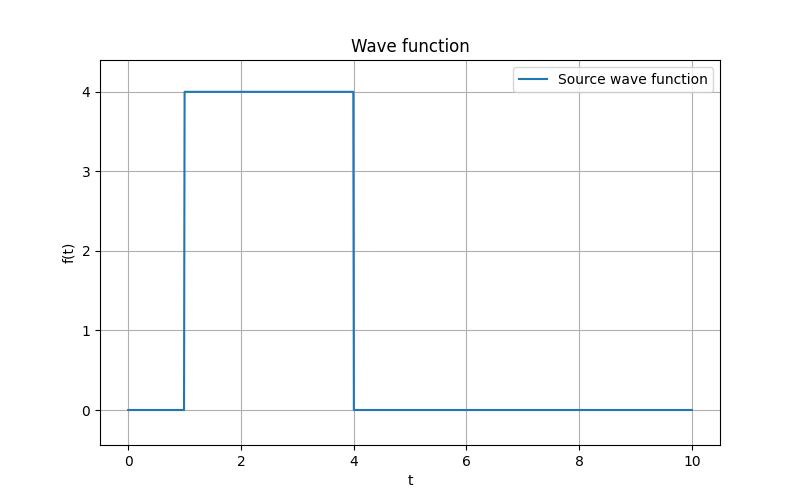
\includegraphics[width=\textwidth]{../results/second/\num/wave_func.png}
    \caption{Функция $g(t)$ с параметрами $a = \a$, $t_1 = \from$, $t_2 = \to$}
    \label{fig:wave_func_\num}
\end{figure}

\begin{figure}[ht!]
    \centering
    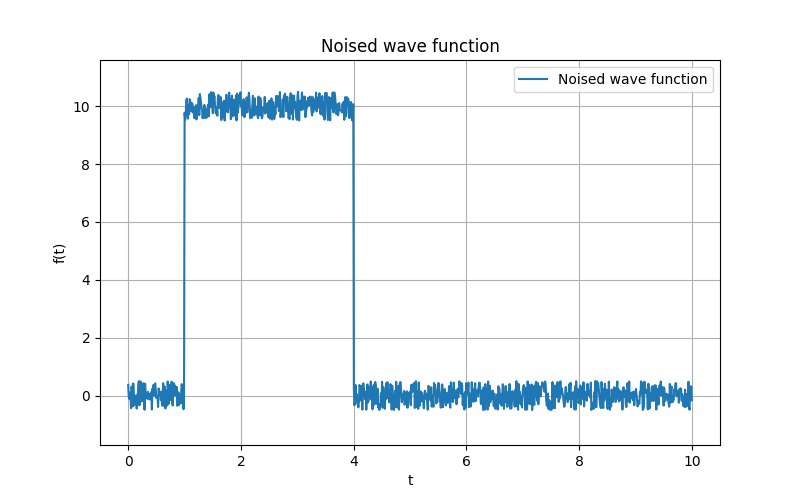
\includegraphics[width=\textwidth]{../results/second/\num/noised_wave_func.png}
    \caption{Функция $u(t)$ с параметрами $b = \b$, $c = \c$, $d = \d$}
    \label{fig:noised_wave_func_\num}
\end{figure}

\FloatBarrier
\subsubsection{Применение фильтра}

Рассмотрим фильтрованную функцию $u'(t)$, которая получается применением линейного фильтра первого порядка с $T = \T$ (см. рисунок \ref{fig:noised_wave_func_filtered_\num}).

\begin{figure}[ht!]
    \centering
    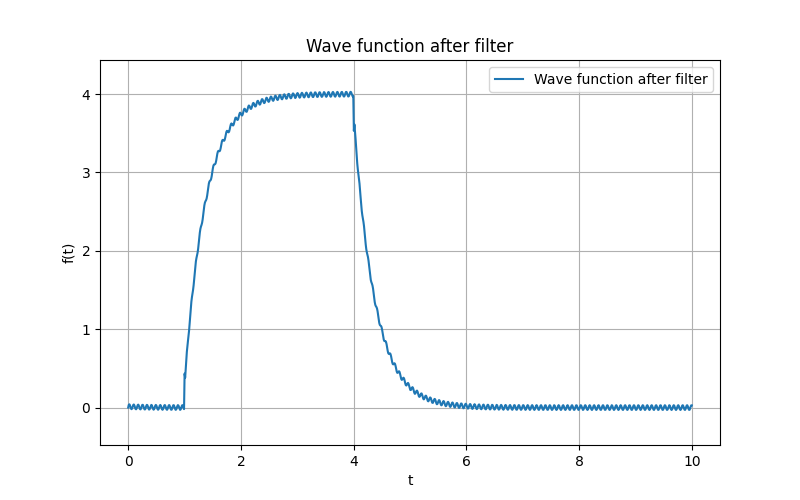
\includegraphics[width=\textwidth]{../results/second/\num/noised_wave_func_filtered.png}
    \caption{Функция $u'(t)$ после применения фильтра}
    \label{fig:noised_wave_func_filtered_\num}
\end{figure}

Видим, что функция после фильтрации стала более гладкой, фронт и спад стали менее выраженными. 
Это связано с тем, что фильтр убирает высокочастотные компоненты функции. Убедиться в этом можно 
рассмотрев АЧХ данного фильтра (см. рисунок \ref{fig:filter_frequency_response_\num}).

\FloatBarrier
\subsubsection{Аплитудно-частотная характеристика фильтра}
\begin{figure}[ht!]
    \centering
    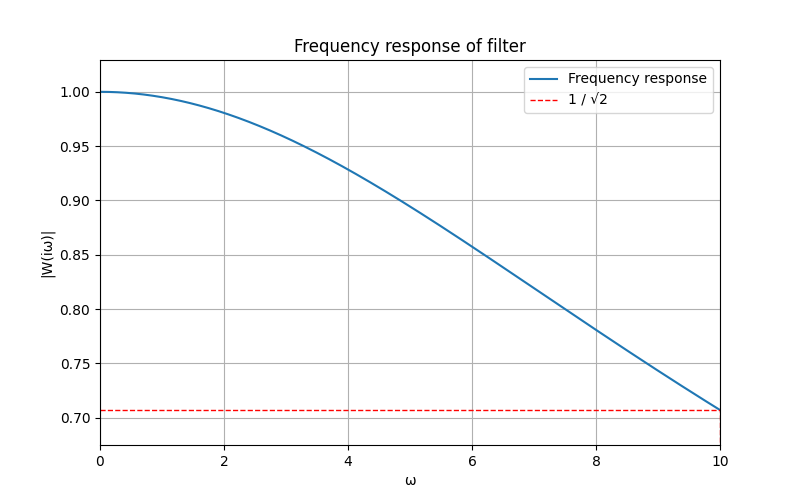
\includegraphics[width=\textwidth]{../results/second/\num/filter_frequency_response.png}
    \caption{АЧХ фильтра первого порядка при $T = \T$}
    \label{fig:filter_frequency_response_\num}
\end{figure}

На графике также отмечено значение $\omega_c$ -- \textit{частоты среза} $|W(i\omega_c)| = \frac{1}{\sqrt{2}}$, по нему можно судить о том, какие частоты будут \textit{усиливаться}, а какие \textit{подавляться}. 
Для фильтра первого порядка это значение равно $\omega_c = \frac{1}{T}$. Таким образом, делаем вывод, что все частоты, 
большие $\frac{1}{\T} = \fpeval{1/ \T}$ будут подавляться, что соответствует значению на графике. 

\FloatBarrier
\subsubsection{Результаы фильтрации}
Сравнительный график исходной функции и функции после фильтрации представлен на рисунке \ref{fig:wave_func_cmp_\num}.

\begin{figure}[ht!]
    \centering
    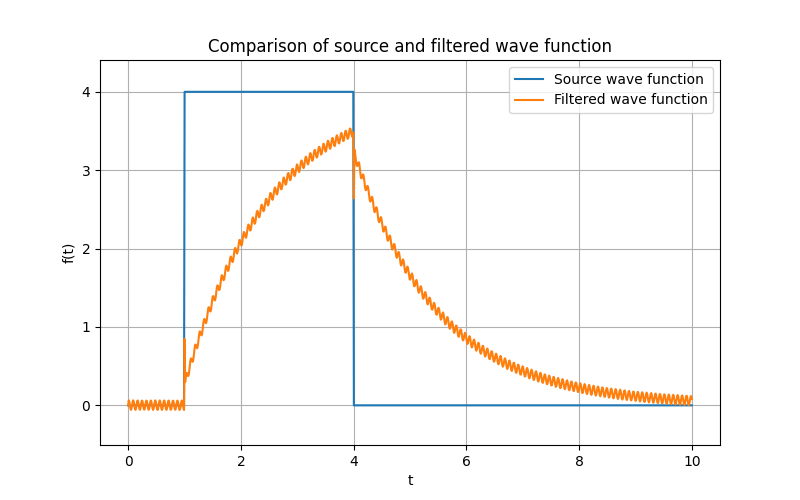
\includegraphics[width=\textwidth]{../results/second/\num/wave_func_cmp.png}
    \caption{Сравнение функции $g(t)$ и $u'(t)$}
    \label{fig:wave_func_cmp_\num}
\end{figure}

Образ исходной функции и функции после фильтрации приведены на рисунках \ref{fig:wave_func_image_\num}~и~\ref{fig:noised_wave_func_filtered_image_\num}.
Графики модулей соответствующих функций приведены на рисунках~\ref{fig:wave_func_image_abs_\num}~и~\ref{fig:noised_wave_func_filtered_image_abs_\num}, их 
сравнительный график -- на рисунке~\ref{fig:wave_func_image_cmp_\num}.

\begin{figure}[ht!]
    \centering
    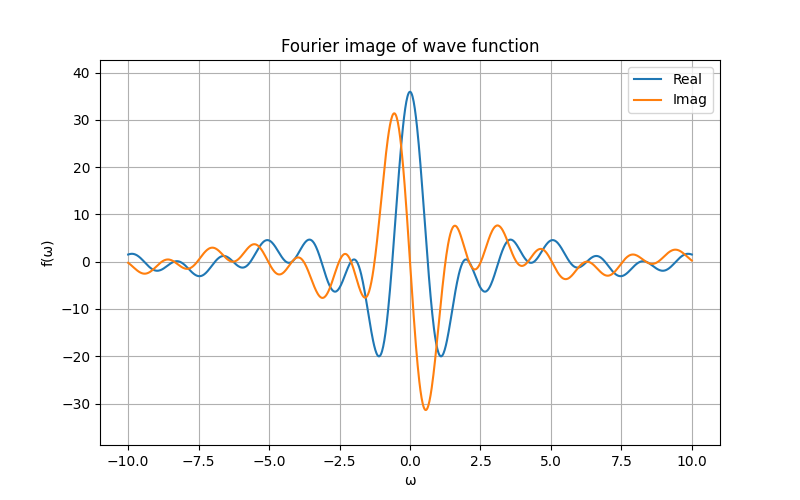
\includegraphics[width=\textwidth]{../results/second/\num/wave_func_image.png}
    \caption{Образ исходной функции $u(t)$.}
    \label{fig:wave_func_image_\num}
\end{figure}

\begin{figure}[ht!]
    \centering
    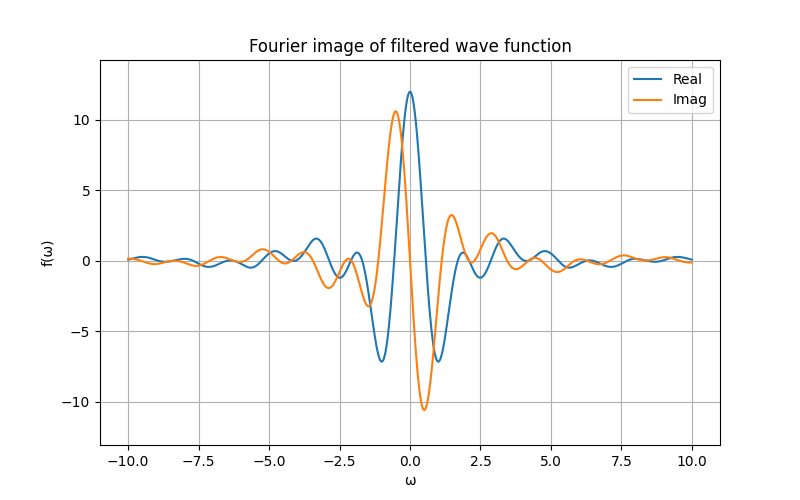
\includegraphics[width=\textwidth]{../results/second/\num/noised_wave_func_filtered_image.png}
    \caption{Образ фильтрованной функции $u'(t)$.}
    \label{fig:noised_wave_func_filtered_image_\num}
\end{figure}

\begin{figure}[ht!]
    \centering
    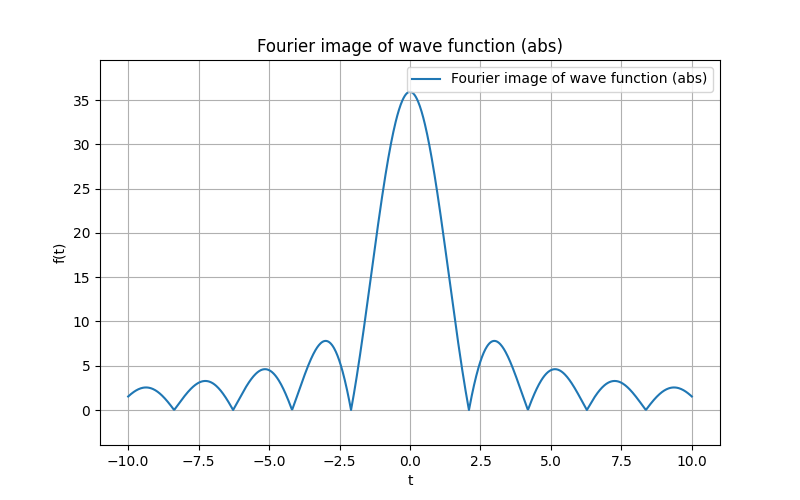
\includegraphics[width=\textwidth]{../results/second/\num/wave_func_image_abs.png}
    \caption{Модуль образа исходной функции $u(t)$.}
    \label{fig:wave_func_image_abs_\num}
\end{figure}

\begin{figure}[ht!]
    \centering
    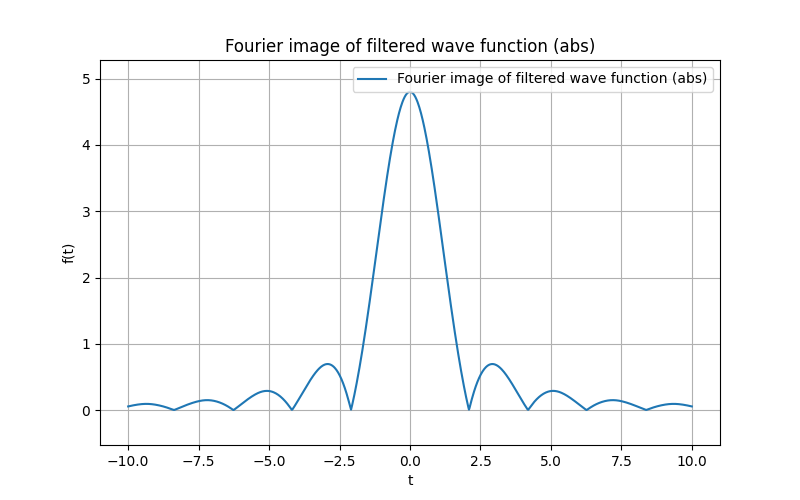
\includegraphics[width=\textwidth]{../results/second/\num/noised_wave_func_filtered_image_abs.png}
    \caption{Модуль образа фильтрованной функции $u'(t)$.}
    \label{fig:noised_wave_func_filtered_image_abs_\num}
\end{figure}

\begin{figure}[ht!]
    \centering
    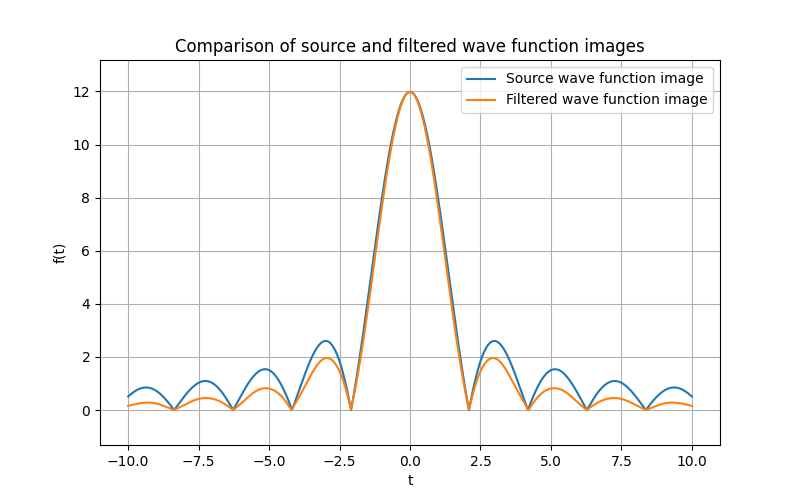
\includegraphics[width=\textwidth]{../results/second/\num/wave_func_image_cmp.png}
    \caption{Сравнение модулей образов исходной и фильтрованной функций.}
    \label{fig:wave_func_image_cmp_\num}
\end{figure}

На графиках модуля исходного и фильтрованного сигнала видно, что фильтр убирает высокочастотные компоненты, что и приводит к сглаживанию функции.

\FloatBarrier
\def\num{2}
\def\T{0.3}
Рассмотрим линейный фильтр первого порядка при $T = \T$ (см. рисунок \ref{fig:noised_wave_func_filtered_\num}).

\begin{figure}[ht!]
    \centering
    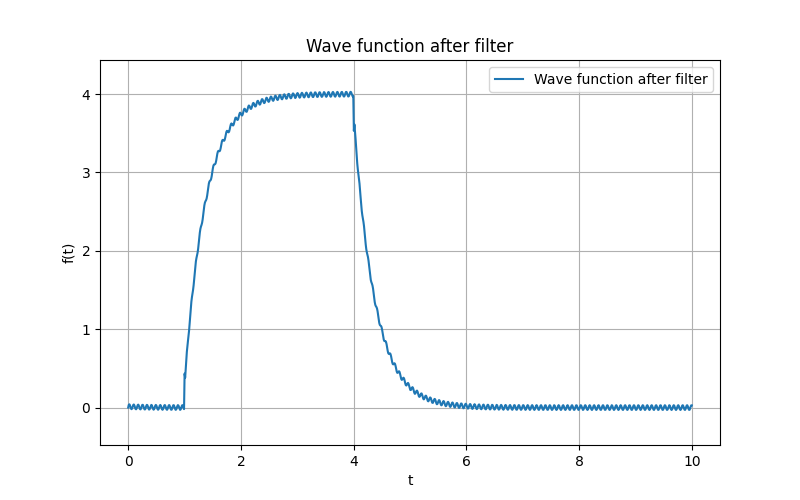
\includegraphics[width=\textwidth]{../results/second/\num/noised_wave_func_filtered.png}
    \caption{Функция $u'(t)$ после применения фильтра}
    \label{fig:noised_wave_func_filtered_\num}
\end{figure}
В данном случае фронт и спад стали более резкими, функция стала больше похожа на исходную. 
АЧХ данного фильтра представлена на рисунке \ref{fig:filter_frequency_response_\num}.

\begin{figure}[ht!]
    \centering
    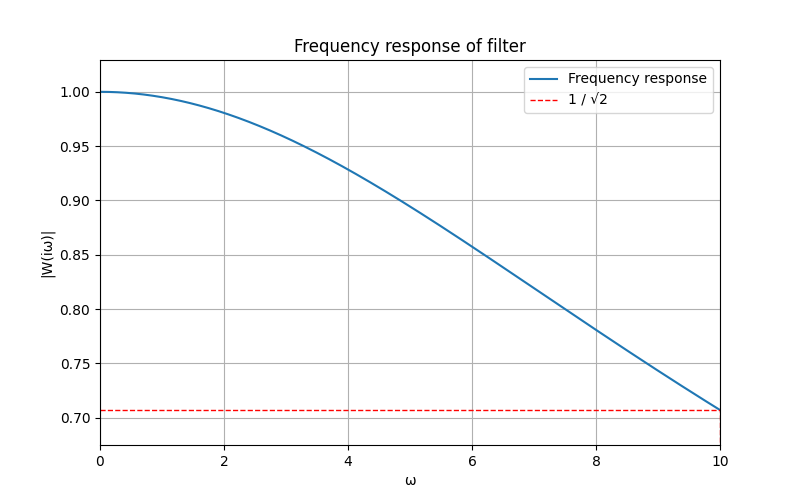
\includegraphics[width=\textwidth]{../results/second/\num/filter_frequency_response.png}
    \caption{АЧХ фильтра первого порядка при $T = \T$}
    \label{fig:filter_frequency_response_\num}
\end{figure}
В данном случае будут подавляться частоты большие $\frac{1}{\T} = \fpeval{round(1/ \T, 3)}$, что значит, что функция лучше повторяет исходную,
по сравнению с прошлой. 

Сравнительный график исходной функции и функции после фильтрации представлен на рисунке \ref{fig:wave_func_cmp_\num}.

Образ исходной функции и функции после фильтрации приведены на рисунках \ref{fig:wave_func_image_\num}~и~\ref{fig:noised_wave_func_filtered_image_\num}.
Графики модулей соответствующих функций приведены на рисунках~\ref{fig:wave_func_image_abs_\num}~и~\ref{fig:noised_wave_func_filtered_image_abs_\num}, их 
сравнительный график -- на рисунке~\ref{fig:wave_func_image_cmp_\num}.

\begin{figure}[ht!]
    \centering
    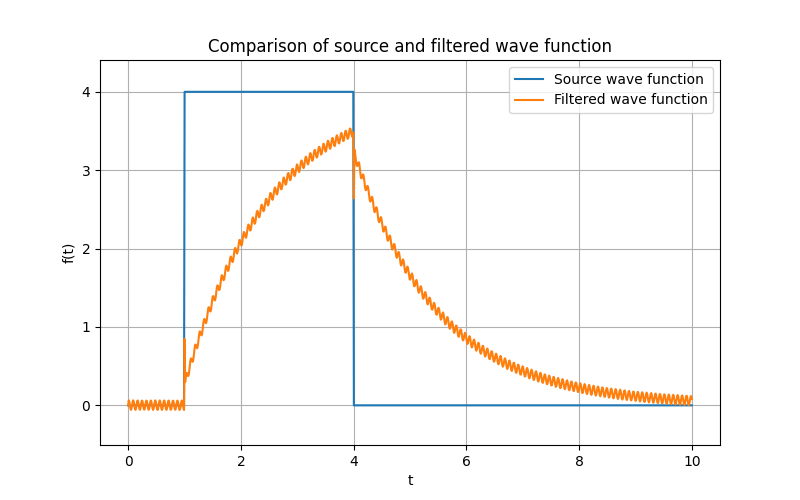
\includegraphics[width=\textwidth]{../results/second/\num/wave_func_cmp.png}
    \caption{Сравнение функции $g(t)$ и $u'(t)$}
    \label{fig:wave_func_cmp_\num}
\end{figure}

\begin{figure}[ht!]
    \centering
    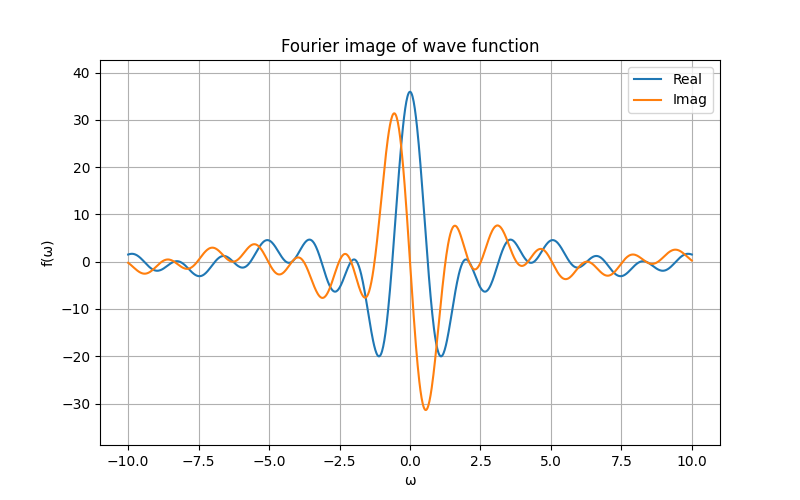
\includegraphics[width=\textwidth]{../results/second/\num/wave_func_image.png}
    \caption{Образ исходной функции $u(t)$.}
    \label{fig:wave_func_image_\num}
\end{figure}

\begin{figure}[ht!]
    \centering
    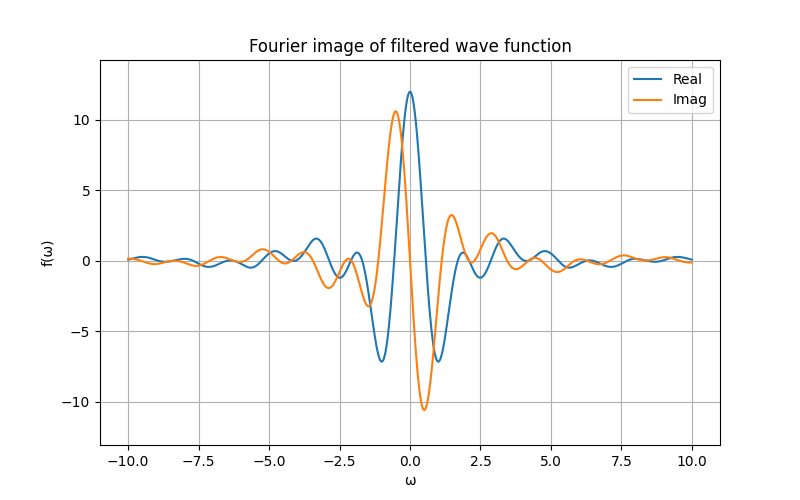
\includegraphics[width=\textwidth]{../results/second/\num/noised_wave_func_filtered_image.png}
    \caption{Образ фильтрованной функции $u'(t)$.}
    \label{fig:noised_wave_func_filtered_image_\num}
\end{figure}

\begin{figure}[ht!]
    \centering
    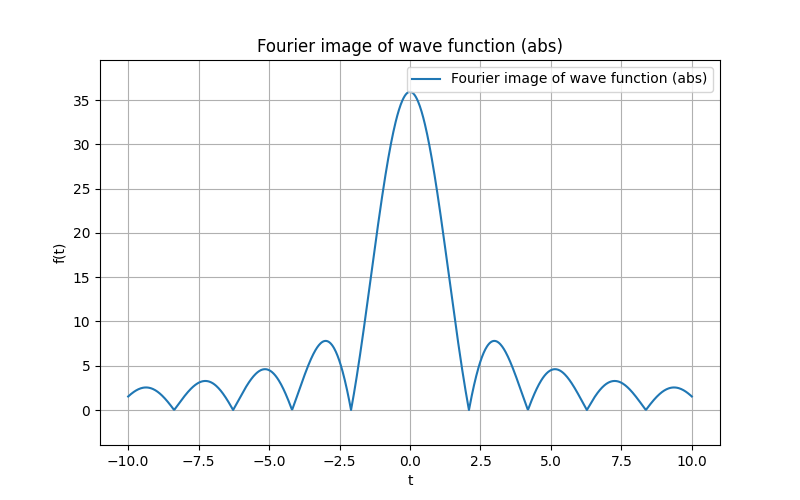
\includegraphics[width=\textwidth]{../results/second/\num/wave_func_image_abs.png}
    \caption{Модуль образа исходной функции $u(t)$.}
    \label{fig:wave_func_image_abs_\num}
\end{figure}

\begin{figure}[ht!]
    \centering
    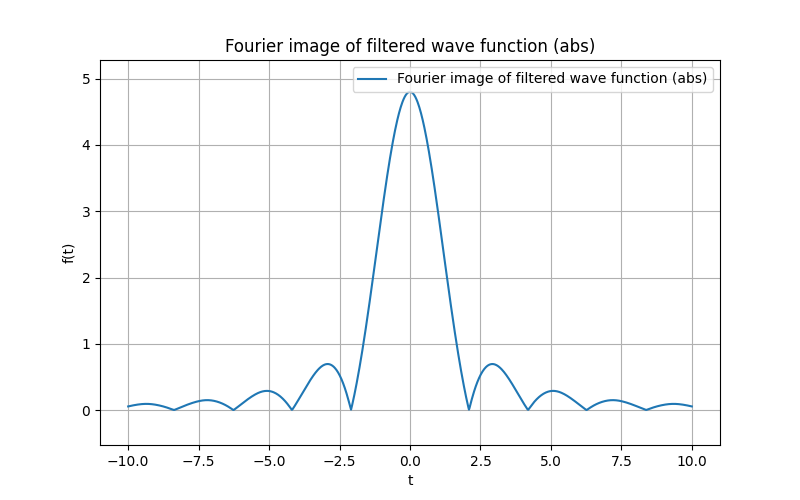
\includegraphics[width=\textwidth]{../results/second/\num/noised_wave_func_filtered_image_abs.png}
    \caption{Модуль образа фильтрованной функции $u'(t)$.}
    \label{fig:noised_wave_func_filtered_image_abs_\num}
\end{figure}

\begin{figure}[ht!]
    \centering
    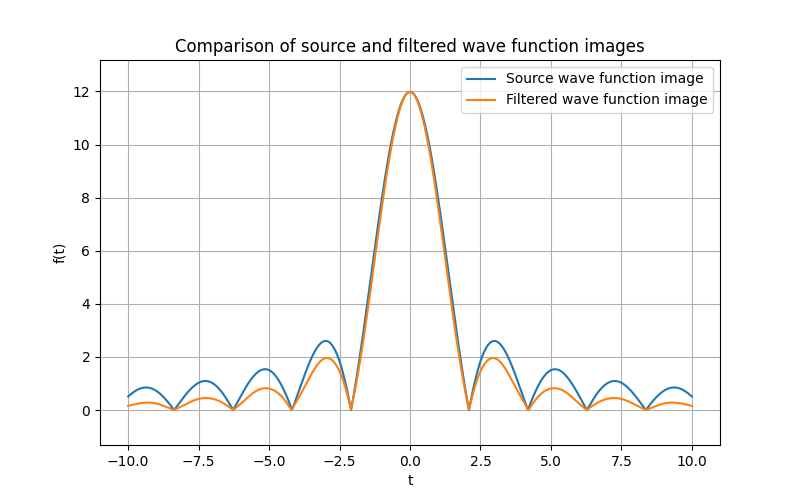
\includegraphics[width=\textwidth]{../results/second/\num/wave_func_image_cmp.png}
    \caption{Сравнение модулей образов исходной и фильтрованной функций.}
    \label{fig:wave_func_image_cmp_\num}
\end{figure}


\FloatBarrier
\def\num{3}
\def\T{0.1}
Также посмотрим на фильтр с параметром $T = \T$ (см. рисунок \ref{fig:noised_wave_func_filtered_\num}).
\begin{figure}[ht!]
    \centering
    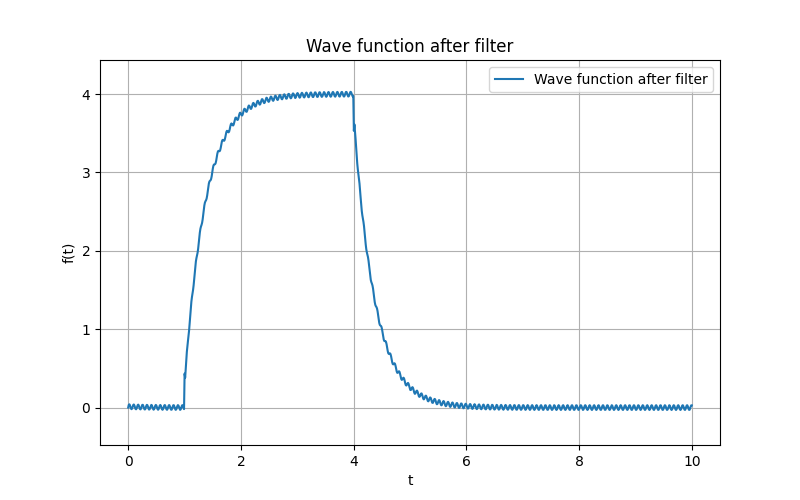
\includegraphics[width=\textwidth]{../results/second/\num/noised_wave_func_filtered.png}
    \caption{Функция $u'(t)$ после применения фильтра}
    \label{fig:noised_wave_func_filtered_\num}
\end{figure}
Теперь функция стала еще более похожей на исходную квадратную волну, но в фильтрованной функции 
стали проявляться шумы из исходной функции. 
АЧХ данного фильтра представлена на рисунке \ref{fig:filter_frequency_response_\num}.

\begin{figure}[ht!]
    \centering
    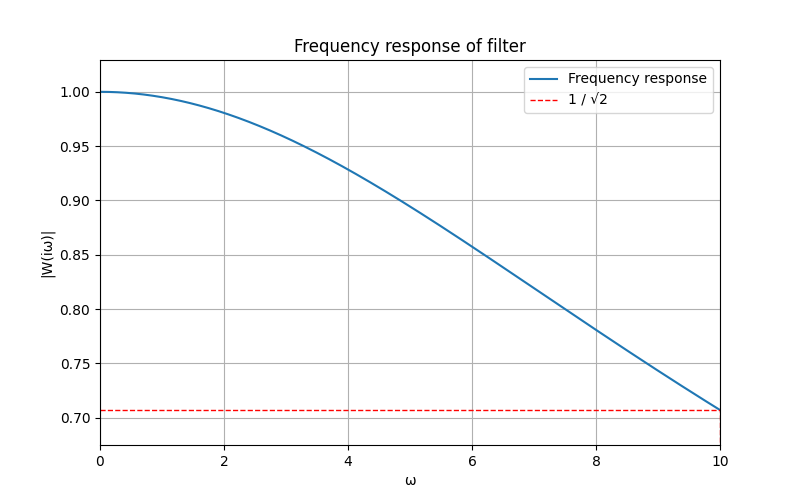
\includegraphics[width=\textwidth]{../results/second/\num/filter_frequency_response.png}
    \caption{АЧХ фильтра первого порядка при $T = \T$}
    \label{fig:filter_frequency_response_\num}
\end{figure}

Сравнительный график исходной функции и функции после фильтрации представлен на рисунке \ref{fig:wave_func_cmp_\num}.

\begin{figure}[ht!]
    \centering
    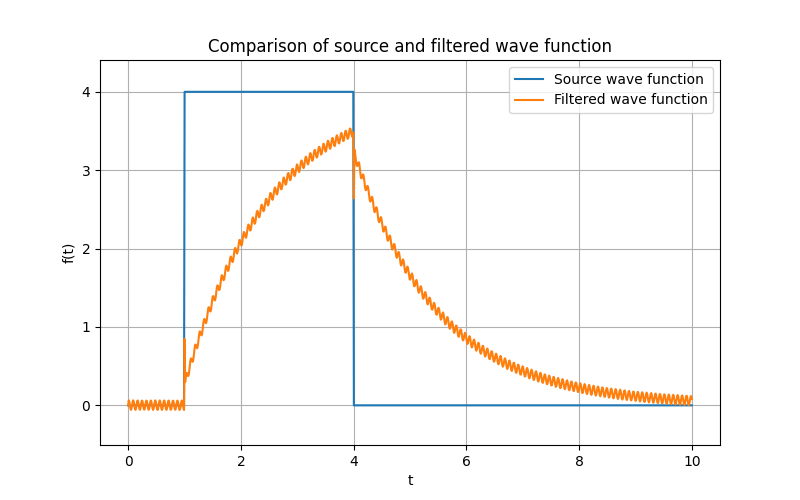
\includegraphics[width=\textwidth]{../results/second/\num/wave_func_cmp.png}
    \caption{Сравнение функции $g(t)$ и $u'(t)$}
    \label{fig:wave_func_cmp_\num}
\end{figure}

Можем сделать вывод, что при увеличении постоянной времени $T$ фильтра, функция становится более гладкой,
при этом меньше похожей на исходную. 

Образ исходной функции и функции после фильтрации приведены на рисунках \ref{fig:wave_func_image_\num}~и~\ref{fig:noised_wave_func_filtered_image_\num}.
Графики модулей соответствующих функций приведены на рисунках~\ref{fig:wave_func_image_abs_\num}~и~\ref{fig:noised_wave_func_filtered_image_abs_\num}, их 
сравнительный график -- на рисунке~\ref{fig:wave_func_image_cmp_\num}.

\begin{figure}[ht!]
    \centering
    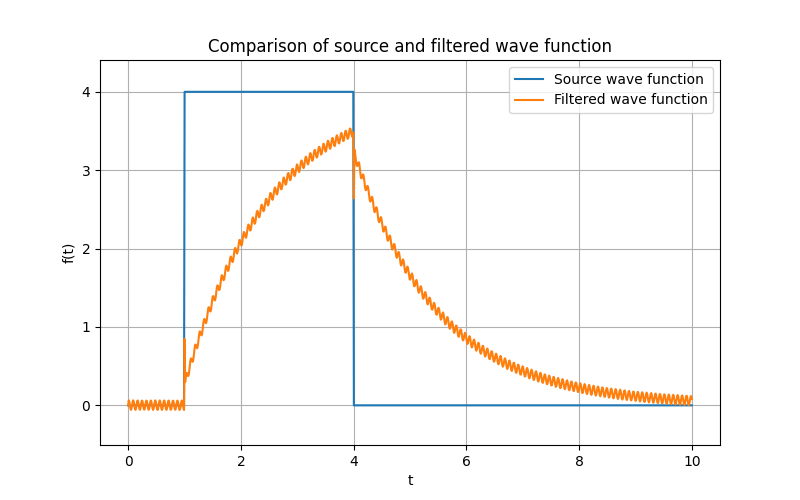
\includegraphics[width=\textwidth]{../results/second/\num/wave_func_cmp.png}
    \caption{Сравнение функции $g(t)$ и $u'(t)$}
    \label{fig:wave_func_cmp_\num}
\end{figure}

\begin{figure}[ht!]
    \centering
    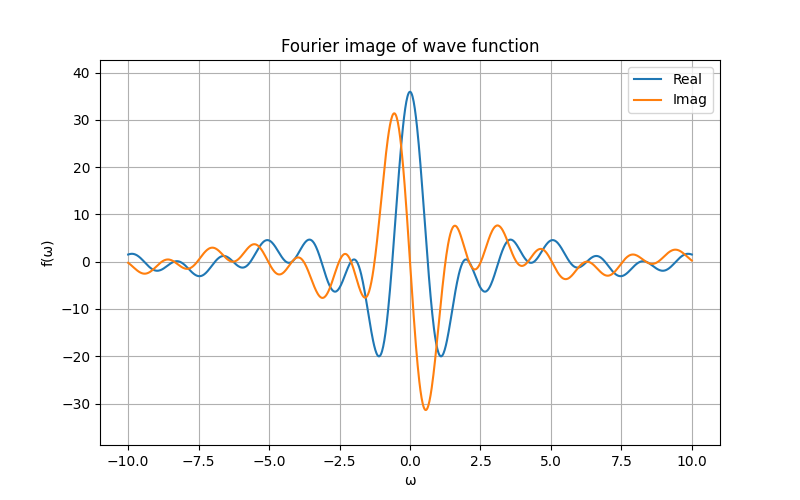
\includegraphics[width=\textwidth]{../results/second/\num/wave_func_image.png}
    \caption{Образ исходной функции $u(t)$.}
    \label{fig:wave_func_image_\num}
\end{figure}

\begin{figure}[ht!]
    \centering
    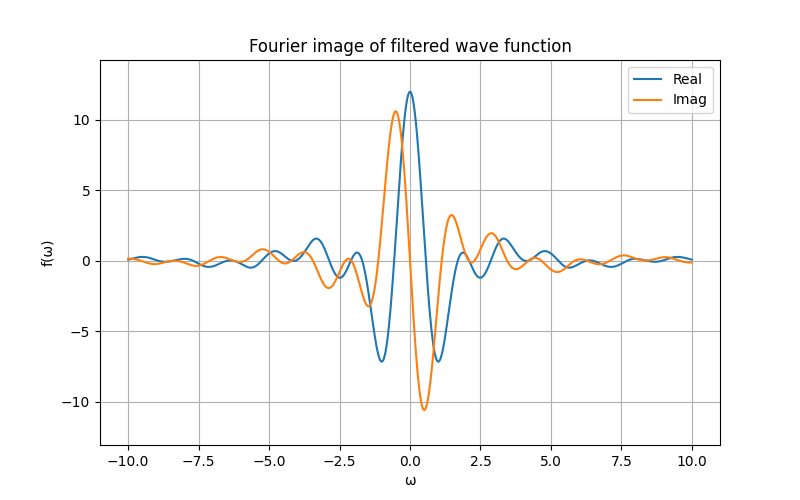
\includegraphics[width=\textwidth]{../results/second/\num/noised_wave_func_filtered_image.png}
    \caption{Образ фильтрованной функции $u'(t)$.}
    \label{fig:noised_wave_func_filtered_image_\num}
\end{figure}

\begin{figure}[ht!]
    \centering
    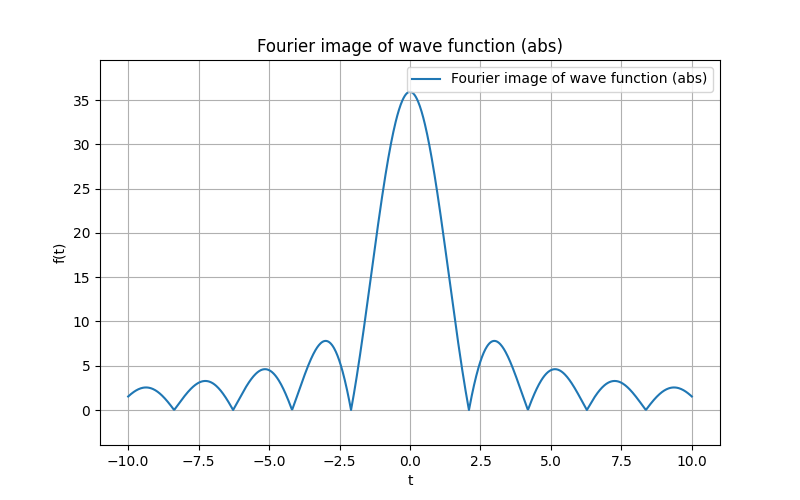
\includegraphics[width=\textwidth]{../results/second/\num/wave_func_image_abs.png}
    \caption{Модуль образа исходной функции $u(t)$.}
    \label{fig:wave_func_image_abs_\num}
\end{figure}

\begin{figure}[ht!]
    \centering
    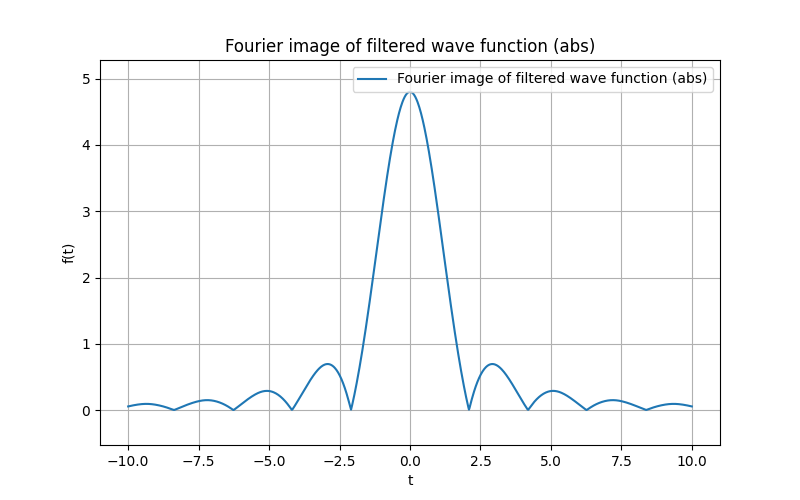
\includegraphics[width=\textwidth]{../results/second/\num/noised_wave_func_filtered_image_abs.png}
    \caption{Модуль образа фильтрованной функции $u'(t)$.}
    \label{fig:noised_wave_func_filtered_image_abs_\num}
\end{figure}

\begin{figure}[ht!]
    \centering
    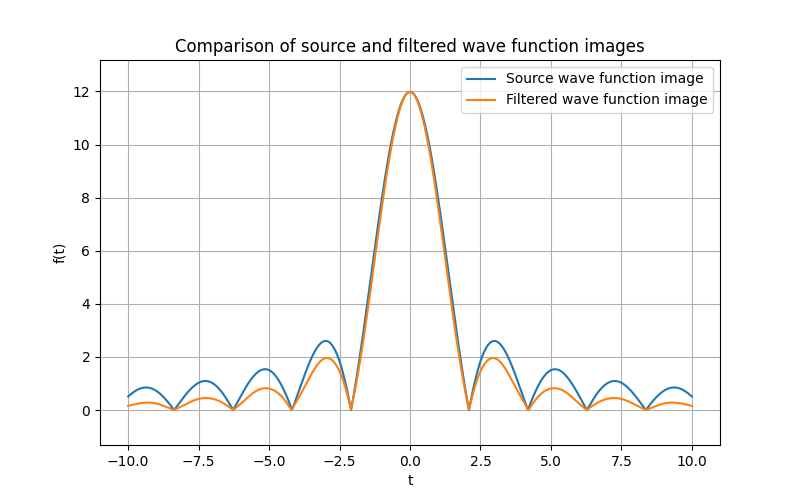
\includegraphics[width=\textwidth]{../results/second/\num/wave_func_image_cmp.png}
    \caption{Сравнение модулей образов исходной и фильтрованной функций.}
    \label{fig:wave_func_image_cmp_\num}
\end{figure}


\FloatBarrier
\subsubsection{Зависимость эффективности фильтрации от параметра a}
\def\T{0.3}
Для исследования данной зависимости рассмотрим функцию $g(t)$ при различных значениях параметра $a$ 
при фильтрации линейным фильтром первого порядка с $T = \T$. 

\def\num{4}
\def\a{10}
Рассмотрим функцию $g(t)$ при параметрах $a=\a$, $t_1 = \from$, $t_2 = \to$ ~(см. рисунок~\ref{fig:wave_func_\num}) 
и ее \textit{зашумленную} версию $u(t)$ с параметрами $b = \b$, $c = \c$, $d = \d$ ~(см. рисунок~\ref{fig:noised_wave_func_\num}).
на промежутке $[0,\L]$. 

\begin{figure}[ht!]
    \centering
    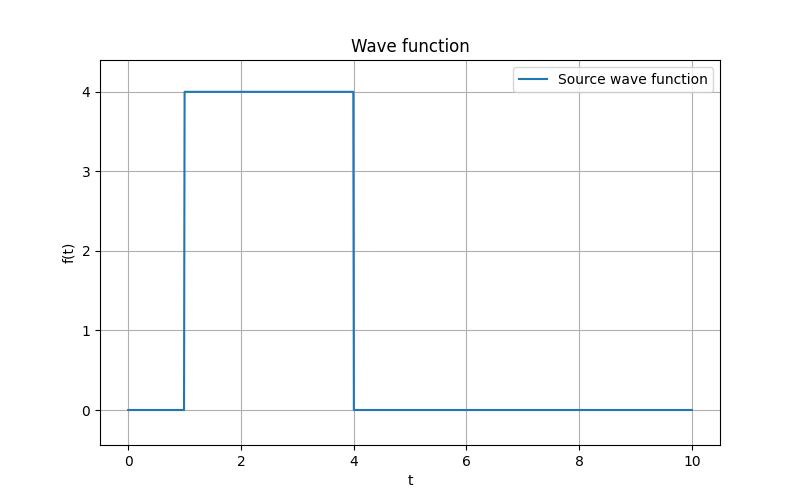
\includegraphics[width=\textwidth]{../results/second/\num/wave_func.png}
    \caption{Функция $g(t)$ с параметрами $a = \a$, $t_1 = \from$, $t_2 = \to$}
    \label{fig:wave_func_\num}
\end{figure}

\begin{figure}[ht!]
    \centering
    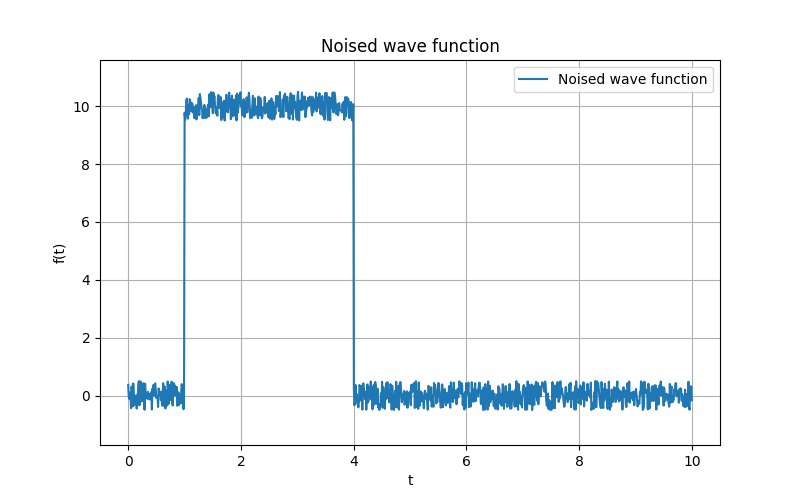
\includegraphics[width=\textwidth]{../results/second/\num/noised_wave_func.png}
    \caption{Функция $u(t)$ с параметрами $b = \b$, $c = \c$, $d = \d$}
    \label{fig:noised_wave_func_\num}
\end{figure}

Результат фильтрации с помощью линейного фильтра первого порядка с $T = \T$ (см. рисунок \ref{fig:noised_wave_func_filtered_\num}).
Сравнительные графики исходной функции и функции после фильтрации представлены на рисунке \ref{fig:wave_func_cmp_\num}.

\begin{figure}[ht!]
    \centering
    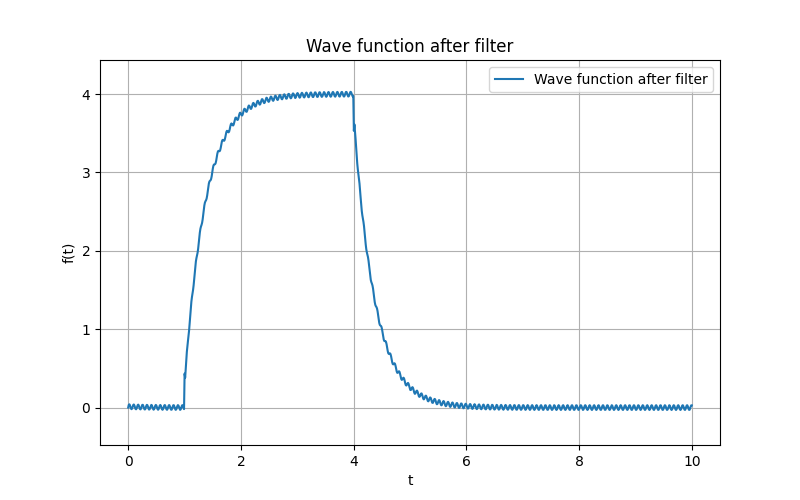
\includegraphics[width=\textwidth]{../results/second/\num/noised_wave_func_filtered.png}
    \caption{Функция $u'(t)$ после применения фильтра}
    \label{fig:noised_wave_func_filtered_\num}
\end{figure}

\begin{figure}[ht!]
    \centering
    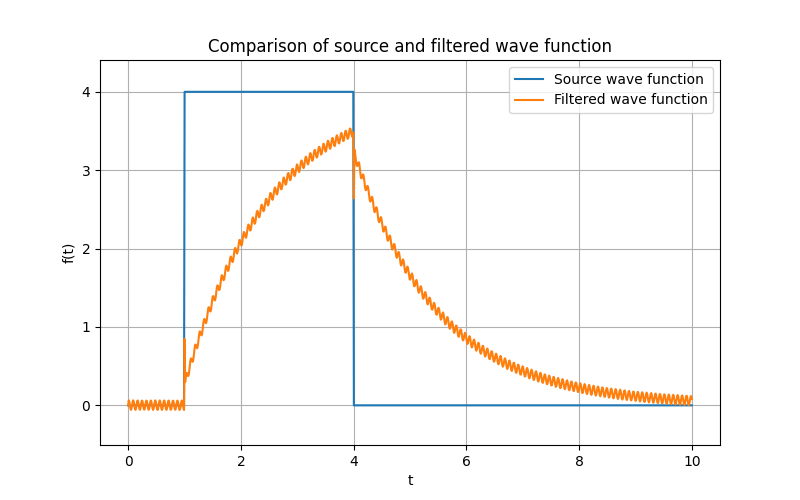
\includegraphics[width=\textwidth]{../results/second/\num/wave_func_cmp.png}
    \caption{Сравнение функции $g(t)$ и $u'(t)$}
    \label{fig:wave_func_cmp_\num}
\end{figure}

Результат практически не отличается от предыдущего случая. Функция стала более гладкой, но при этом
менее похожей на исходную. Фронт и спад так же завалены. 

\def\num{5}
\def\a{30}
Рассмотрим функцию $g(t)$ при параметрах $a=\a$, $t_1 = \from$, $t_2 = \to$ ~(см. рисунок~\ref{fig:wave_func_\num}) 
и ее \textit{зашумленную} версию $u(t)$ с параметрами $b = \b$, $c = \c$, $d = \d$ ~(см. рисунок~\ref{fig:noised_wave_func_\num}).
на промежутке $[0,\L]$. 

\begin{figure}[ht!]
    \centering
    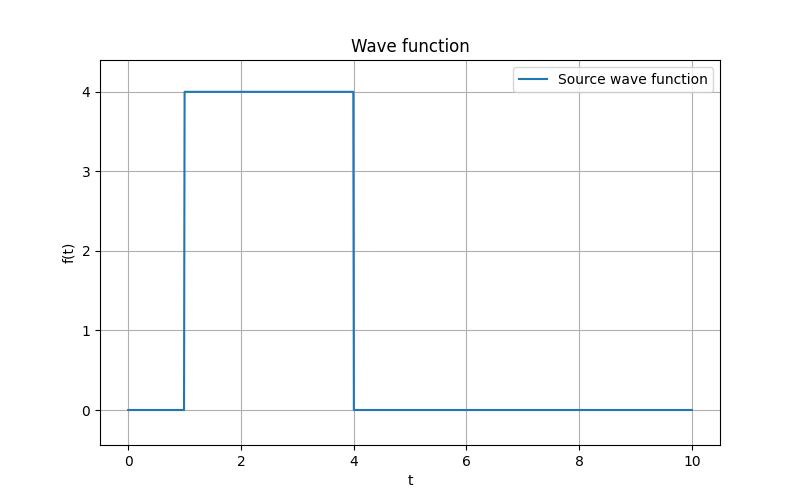
\includegraphics[width=\textwidth]{../results/second/\num/wave_func.png}
    \caption{Функция $g(t)$ с параметрами $a = \a$, $t_1 = \from$, $t_2 = \to$}
    \label{fig:wave_func_\num}
\end{figure}

\begin{figure}[ht!]
    \centering
    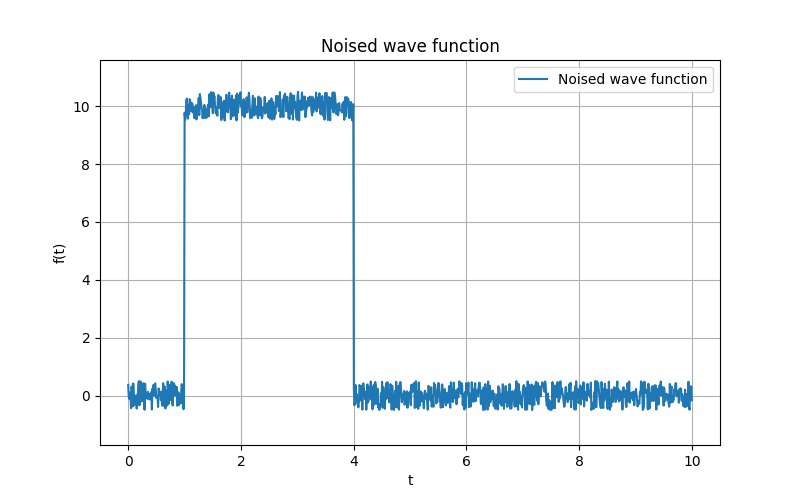
\includegraphics[width=\textwidth]{../results/second/\num/noised_wave_func.png}
    \caption{Функция $u(t)$ с параметрами $b = \b$, $c = \c$, $d = \d$}
    \label{fig:noised_wave_func_\num}
\end{figure}

Результат фильтрации с помощью линейного фильтра первого порядка с $T = \T$ (см. рисунок \ref{fig:noised_wave_func_filtered_\num}).

\begin{figure}[ht!]
    \centering
    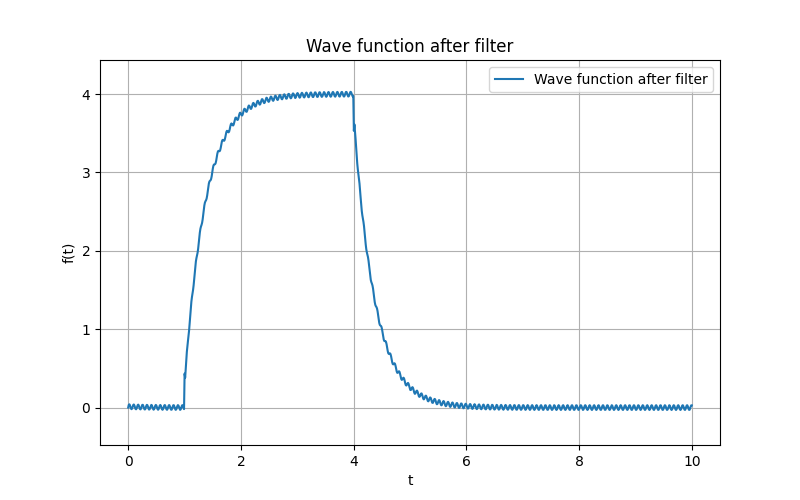
\includegraphics[width=\textwidth]{../results/second/\num/noised_wave_func_filtered.png}
    \caption{Функция $u'(t)$ после применения фильтра}
    \label{fig:noised_wave_func_filtered_\num}
\end{figure}

\begin{figure}[ht!]
    \centering
    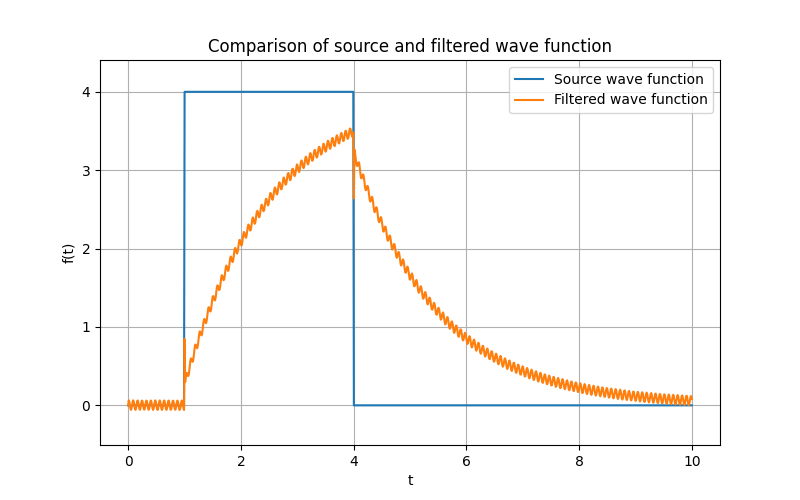
\includegraphics[width=\textwidth]{../results/second/\num/wave_func_cmp.png}
    \caption{Сравнение функции $g(t)$ и $u'(t)$}
    \label{fig:wave_func_cmp_\num}
\end{figure}

Ровно как и в прошлый раз -- никаких изменений. Фронт функции выглядит идентично с поправкой на масштаб.
Сравнительные графики исходной функции и функции после фильтрации представлены на рисунке \ref{fig:wave_func_cmp_\num}.

Можно сделать вывод, что параметр $a$ не влияет на эффективность фильтрации линейным фильтром первого порядка. 
Связано это с тем, что, фильтр первого порядка лишь \textit{масштабирует} функцию согласно его АЧХ. 


\FloatBarrier
\subsection{Специальный фильтр}

Будем рассматривать линейный фильтр второго порядка вида: 
\begin{equation}
    W_2(p) = \frac{(T_1p + 1)^2}{(T_2p + 1)(T_3p + 1)} = \frac{T_1^2p^2 + 2T_1p + 1}{T_2T_3p^2 + (T_2 + T_3)p + 1}
\end{equation}

Для того, чтобы подобрать коэффициенты $T_1$, $T_2$, $T_3$, я рассмотрел данный фильтр в виде произведения двух фильтров первого порядка. 
В ходе рассмотрения графиков АЧХ данных фильтров я пришел к выводу, что, можно ввести параметры $w_0$ и $A$ -- частота, на которой происходить фильтрация и коэффициент подавления на этой частоте соответственно.
коэффициенты исходного фильтра получаются следующим образом:
\begin{equation}
    T_1 = \frac{1}{w_0}, \quad T_2 = \frac{A}{w_0}, \quad T_3 = \frac{1}{Aw_0}
    \label{eq:t_params}
\end{equation}

\def\num{6}
\def\a{4}
\def\from{1}
\def\to{4}
\def\b{0}
\def\c{0.4}
\def\d{80}
\def\L{10}
\def\A{30}
\def\Wz{80}
\def\Tf{\fpeval{round(1 / \Wz, 7)}}
\def\Ts{\fpeval{round(\A / \Wz, 7)}}
\def\Tt{\fpeval{round(1 / (\A * \Wz), 7)}}

\subsubsection{Рассматриваемая функция}
Рассмотрим функцию $g(t)$ при параметрах $a=\a$, $t_1 = \from$, $t_2 = \to$ ~(см. рисунок~\ref{fig:wave_func_\num}) 
и ее \textit{зашумленную} версию $u(t)$ с параметрами $b = \b$, $c = \c$, $d = \d$ ~(см. рисунок~\ref{fig:noised_wave_func_\num}).
на промежутке $[0,\L]$. 

\subsubsection{Графики рассматриваемой и зашумленной функции}
\begin{figure}[ht!]
    \centering
    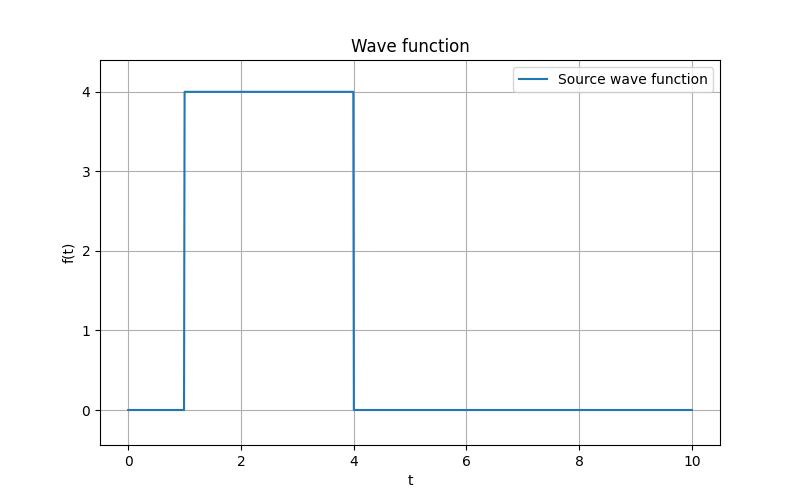
\includegraphics[width=\textwidth]{../results/second/\num/wave_func.png}
    \caption{Функция $g(t)$ с параметрами $a = \a$, $t_1 = \from$, $t_2 = \to$}
    \label{fig:wave_func_\num}
\end{figure}

\begin{figure}[ht!]
    \centering
    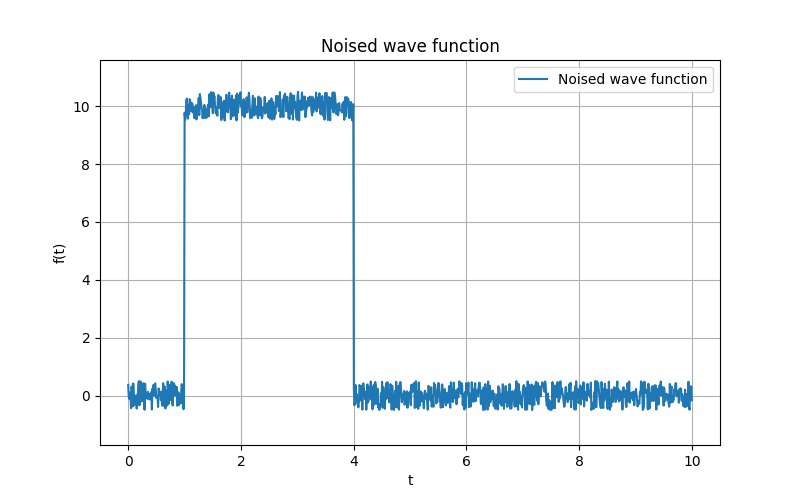
\includegraphics[width=\textwidth]{../results/second/\num/noised_wave_func.png}
    \caption{Функция $u(t)$ с параметрами $b = \b$, $c = \c$, $d = \d$}
    \label{fig:noised_wave_func_\num}
\end{figure}

\FloatBarrier
\subsubsection{Применение фильтра}

Рассмотрим фильтрованную функцию $u'(t)$, которая получается применением линейного фильтра второго порядка с $T_1 = \Tf$, $T_2 = \Ts$, $T_3 = \Tt$ (см. рисунок \ref{fig:noised_wave_func_filtered_\num}).
Значения $T_1,~T_2,~T_3$ получены из формул \eqref{eq:t_params} при $w_0 = \Wz$ и $A = \A$.

\begin{figure}[ht!]
    \centering
    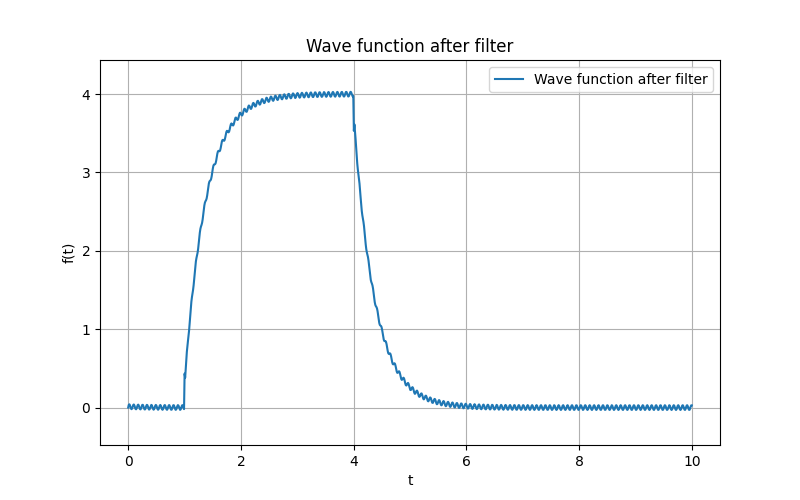
\includegraphics[width=\textwidth]{../results/second/\num/noised_wave_func_filtered.png}
    \caption{Функция $u'(t)$ после применения фильтра}
    \label{fig:noised_wave_func_filtered_\num}
\end{figure}

Видим, что функция после фильтрации стала более гладкой, фронт и спад стали менее выраженными.
Это связано с тем, что фильтр убирает высокочастотные компоненты функции. Убедиться в этом можно 
посмотрев на АЧХ фильтра (см. рисунок \ref{fig:filter_frequency_response_\num} и \ref{fig:filter_frequency_response_log_\num}).

\FloatBarrier
\subsubsection{Амплитудно-частотная характеристика фильтра}
\begin{figure}[ht!]
    \centering
    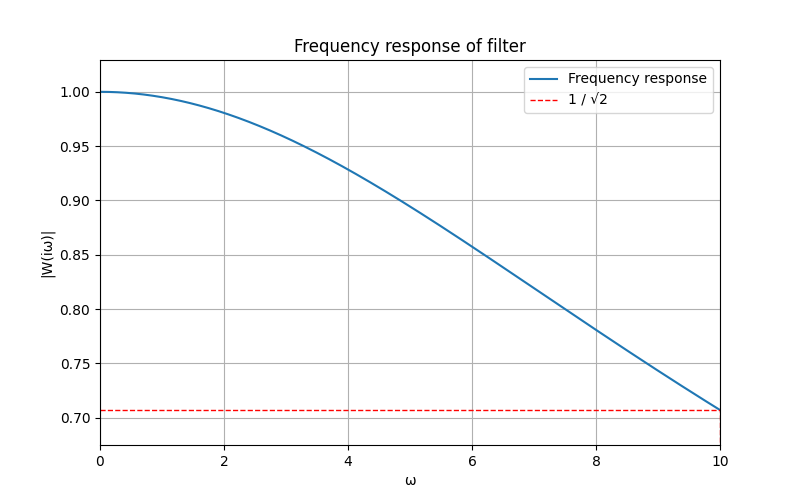
\includegraphics[width=\textwidth]{../results/second/\num/filter_frequency_response.png}
    \caption{АЧХ фильтра второго порядка при $T_1 = \Tf$, $T_2 = \Ts$, $T_3 = \Tt$}
    \label{fig:filter_frequency_response_\num}
\end{figure}

\begin{figure}[ht!]
    \centering
    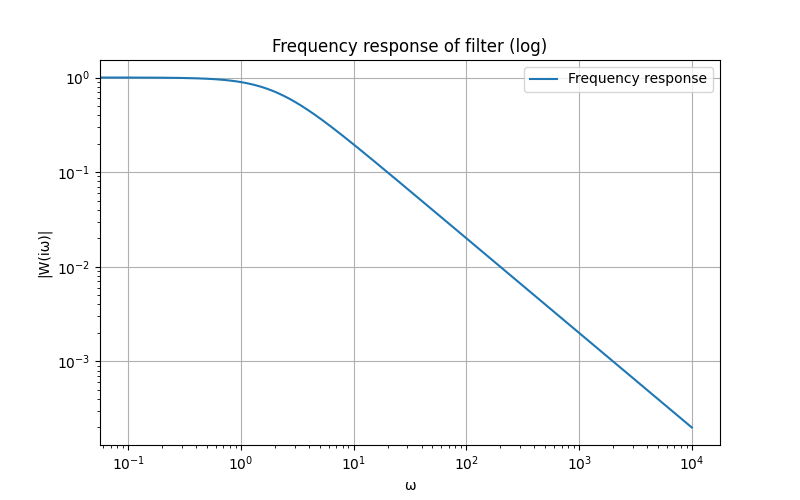
\includegraphics[width=\textwidth]{../results/second/\num/filter_frequency_response_log.png}
    \caption{АЧХ фильтра второго порядка при $T_1 = \Tf$, $T_2 = \Ts$, $T_3 = \Tt$ (логарифмическая шкала)}
    \label{fig:filter_frequency_response_log_\num}
\end{figure}

На логарифмическом графике более заметно, что данный фильтр подавляет частоты в окрестности частоты $w_0 = \Wz$, что и требуется для фильтрации гармонического шума. 
Но, на этом же графике видно, что фильтр, кроме требуемых частот, подавляет довольно большой диапазон частот, что, конечно, сильно сказывается на качестве фильтрации. 
Именно для того, чтобы фильтр минимально срезал нижние частоты, которые необходимы для восстановления исходной функции была выбрана довольно большая частота гармонического шума.

\FloatBarrier
\subsubsection{Результаты фильтрации}
Сравнительный график исходной функции и функции после фильтрации представлен на рисунке \ref{fig:wave_func_cmp_\num}.

\begin{figure}[ht!]
    \centering
    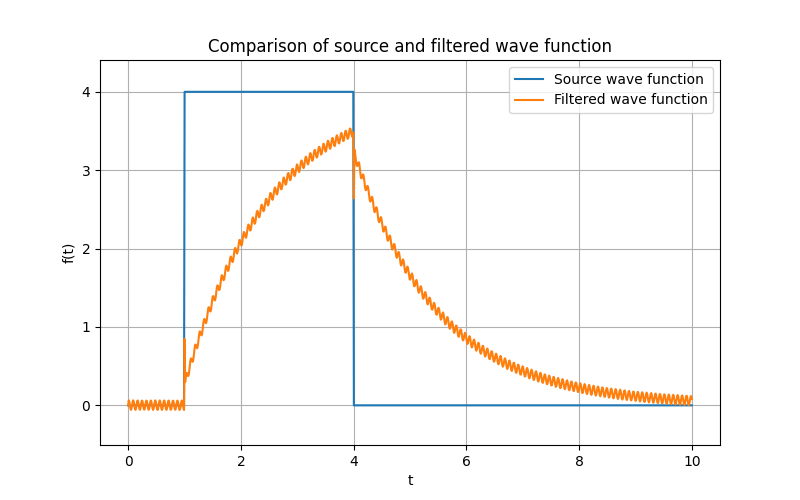
\includegraphics[width=\textwidth]{../results/second/\num/wave_func_cmp.png}
    \caption{Сравнение функции $g(t)$ и $u'(t)$}
    \label{fig:wave_func_cmp_\num}
\end{figure}

Образ исходной функции и функции после фильтрации приведены на рисунках \ref{fig:wave_func_image_\num}~и~\ref{fig:noised_wave_func_filtered_image_\num}.
Графики модулей соответствующих функций приведены на рисунках~\ref{fig:wave_func_image_abs_\num}~и~\ref{fig:noised_wave_func_filtered_image_abs_\num}, их 
сравнительный график -- на рисунке~\ref{fig:wave_func_image_cmp_\num}.

На сравнительном графике (см. рисунок~\ref{fig:wave_func_image_cmp_\num}) видно, что \textit{амплитуда} образа фильтрованного сигнала уменьшается по сравнению 
с образом начальной функции. Результат соответствует АЧХ фильтра (см. рисунок~\ref{fig:filter_frequency_response_\num}).

\begin{figure}[ht!]
    \centering
    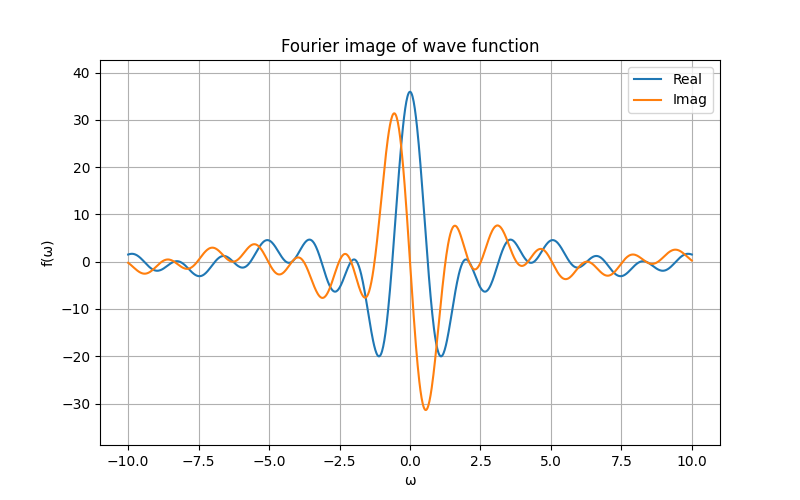
\includegraphics[width=\textwidth]{../results/second/\num/wave_func_image.png}
    \caption{Образ исходной функции $u(t)$.}
    \label{fig:wave_func_image_\num}
\end{figure}

\begin{figure}[ht!]
    \centering
    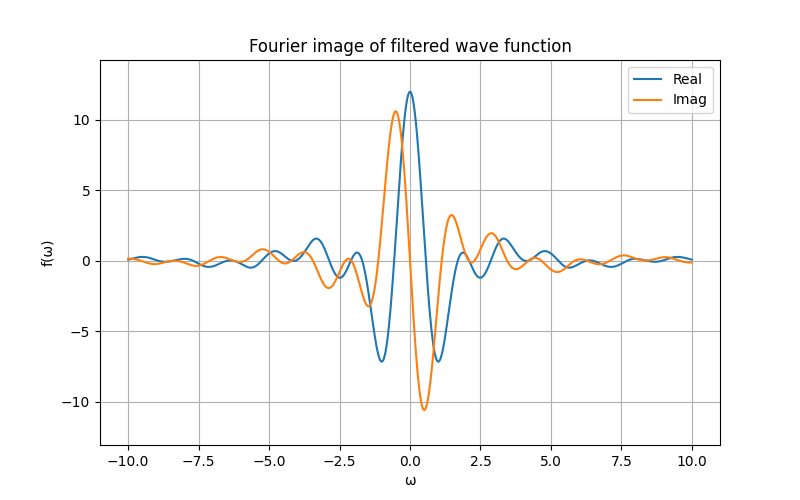
\includegraphics[width=\textwidth]{../results/second/\num/noised_wave_func_filtered_image.png}
    \caption{Образ фильтрованной функции $u'(t)$.}
    \label{fig:noised_wave_func_filtered_image_\num}
\end{figure}

\begin{figure}[ht!]
    \centering
    \includegraphics[width=\textwidth]{../results/second/\num/wave_func_image_abs.png}
    \caption{Модуль образа исходной функции $u(t)$.}
    \label{fig:wave_func_image_abs_\num}
\end{figure}

\begin{figure}[ht!]
    \centering
    \includegraphics[width=\textwidth]{../results/second/\num/noised_wave_func_filtered_image_abs.png}
    \caption{Модуль образа фильтрованной функции $u'(t)$.}
    \label{fig:noised_wave_func_filtered_image_abs_\num}
\end{figure}

\begin{figure}[ht!]
    \centering
    \includegraphics[width=\textwidth]{../results/second/\num/wave_func_image_cmp.png}
    \caption{Сравнение модулей образов исходной и фильтрованной функций.}
    \label{fig:wave_func_image_cmp_\num}
\end{figure}

\FloatBarrier
\subsubsection{Фильтрация шума меньшей частоты}

\def\num{7}
\def\a{4}
\def\from{1}
\def\to{4}
\def\b{0}
\def\c{0.4}
\def\d{20}
\def\L{10}
\def\A{30}
\def\Wz{20}
\def\Tf{\fpeval{round(1 / \Wz, 7)}}
\def\Ts{\fpeval{round(\A / \Wz, 7)}}
\def\Tt{\fpeval{round(1 / (\A * \Wz), 7)}}

Теперь рассмотрим функцию с гармоническом шумом меньшей частоты, чем в предыдущем случае: 
$g(t)$ при параметрах $a=\a$, $t_1 = \from$, $t_2 = \to$ ~(см. рисунок~\ref{fig:wave_func_\num}) 
и ее \textit{зашумленную} версию $u(t)$ с параметрами $b = \b$, $c = \c$, $d = \d$ ~(см. рисунок~\ref{fig:noised_wave_func_\num}).
на промежутке $[0,\L]$. 

\begin{figure}[ht!]
    \centering
    \includegraphics[width=\textwidth]{../results/second/\num/wave_func.png}
    \caption{Функция $g(t)$ с параметрами $a = \a$, $t_1 = \from$, $t_2 = \to$}
    \label{fig:wave_func_\num}
\end{figure}

\begin{figure}[ht!]
    \centering
    \includegraphics[width=\textwidth]{../results/second/\num/noised_wave_func.png}
    \caption{Функция $u(t)$ с параметрами $b = \b$, $c = \c$, $d = \d$}
    \label{fig:noised_wave_func_\num}
\end{figure}

Рассмотрим фильтрованную функцию $u'(t)$, которая получается применением линейного фильтра второго порядка с $T_1 = \Tf$, $T_2 = \Ts$, $T_3 = \Tt$ (см. рисунок \ref{fig:noised_wave_func_filtered_\num}).
Значения $T_1,~T_2,~T_3$ получены из формул \eqref{eq:t_params} при $w_0 = \Wz$ и $A = \A$.

\begin{figure}[ht!]
    \centering
    \includegraphics[width=\textwidth]{../results/second/\num/noised_wave_func_filtered.png}
    \caption{Функция $u'(t)$ после применения фильтра}
    \label{fig:noised_wave_func_filtered_\num}
\end{figure}

На рисунке~\ref{fig:noised_wave_func_filtered_\num} видно, что гармонический шум действительно уменьшился, при этом,
фронт и спад функции стали менее выраженными. Это связано с тем, что фильтр убирает не только частоты гармонического шума,
но и некоторый диапазон частот рядом с ним, что и приводит к сглаживанию функции.
Убедить в этом можно посмотрев на графики АЧХ данного фильтра (см. рисунок \ref{fig:filter_frequency_response_\num} и \ref{fig:filter_frequency_response_log_\num}).

\begin{figure}[ht!]
    \centering
    \includegraphics[width=\textwidth]{../results/second/\num/filter_frequency_response.png}
    \caption{АЧХ фильтра второго порядка при $T_1 = \Tf$, $T_2 = \Ts$, $T_3 = \Tt$}
    \label{fig:filter_frequency_response_\num}
\end{figure}

\begin{figure}[ht!]
    \centering
    \includegraphics[width=\textwidth]{../results/second/\num/filter_frequency_response_log.png}
    \caption{АЧХ фильтра второго порядка при $T_1 = \Tf$, $T_2 = \Ts$, $T_3 = \Tt$ (логарифмическая шкала)}
    \label{fig:filter_frequency_response_log_\num}
\end{figure}

Сравнительный график исходной и фильтрованной функции приведен на рисунке~\ref{fig:wave_func_cmp_\num}.
\begin{figure}[ht!]
    \centering
    \includegraphics[width=\textwidth]{../results/second/\num/wave_func_cmp.png}
    \caption{Сравнение функции $g(t)$ и $u'(t)$}
    \label{fig:wave_func_cmp_\num}
\end{figure}

\FloatBarrier
\subsubsection{Фильтрация шума большей частоты}

\def\num{8}
\def\a{4}
\def\from{1}
\def\to{4}
\def\b{0}
\def\c{1}
\def\d{2000}
\def\L{10}
\def\A{300}
\def\Wz{2000}
\def\Tf{\fpeval{round(1 / \Wz, 7)}}
\def\Ts{\fpeval{round(\A / \Wz, 7)}}
\def\Tt{\fpeval{round(1 / (\A * \Wz), 7)}}

Теперь рассмотрим более удачный случай, когда гармонический шум имеет большую частоту. Такую, что
при применении фильтра не будет захватываться диапазон частот, необходимый для восстановления исходной функции.

Рассмотрим функцию $g(t)$ при параметрах $a=\a$, $t_1 = \from$, $t_2 = \to$ ~(см. рисунок~\ref{fig:wave_func_\num}) 
и ее \textit{зашумленную} версию $u(t)$ с параметрами $b = \b$, $c = \c$, $d = \d$ ~(см. рисунок~\ref{fig:noised_wave_func_\num}).
на промежутке $[0,\L]$. 

\begin{figure}[ht!]
    \centering
    \includegraphics[width=\textwidth]{../results/second/\num/wave_func.png}
    \caption{Функция $g(t)$ с параметрами $a = \a$, $t_1 = \from$, $t_2 = \to$}
    \label{fig:wave_func_\num}
\end{figure}

\begin{figure}[ht!]
    \centering
    \includegraphics[width=\textwidth]{../results/second/\num/noised_wave_func.png}
    \caption{Функция $u(t)$ с параметрами $b = \b$, $c = \c$, $d = \d$}
    \label{fig:noised_wave_func_\num}
\end{figure}

Рассмотрим фильтрованную функцию $u'(t)$, которая получается применением линейного фильтра второго порядка с $T_1 = \Tf$, $T_2 = \Ts$, $T_3 = \Tt$ (см. рисунок \ref{fig:noised_wave_func_filtered_\num}).
Значения $T_1,~T_2,~T_3$ получены из формул \eqref{eq:t_params} при $w_0 = \Wz$ и $A = \A$.
АЧХ данного фильтра приведена на рисунках \ref{fig:filter_frequency_response_\num} и \ref{fig:filter_frequency_response_log_\num}.

\begin{figure}[ht!]
    \centering
    \includegraphics[width=\textwidth]{../results/second/\num/noised_wave_func_filtered.png}
    \caption{Функция $u'(t)$ после применения фильтра}
    \label{fig:noised_wave_func_filtered_\num}
\end{figure}

\begin{figure}[ht!]
    \centering
    \includegraphics[width=\textwidth]{../results/second/\num/filter_frequency_response.png}
    \caption{АЧХ фильтра второго порядка при $T_1 = \Tf$, $T_2 = \Ts$, $T_3 = \Tt$}
    \label{fig:filter_frequency_response_\num}
\end{figure}

\begin{figure}[ht!]
    \centering
    \includegraphics[width=\textwidth]{../results/second/\num/filter_frequency_response_log.png}
    \caption{АЧХ фильтра второго порядка при $T_1 = \Tf$, $T_2 = \Ts$, $T_3 = \Tt$ (логарифмическая шкала)}
    \label{fig:filter_frequency_response_log_\num}
\end{figure}

Видно, что гармонический шум практически полностью был убран, при этом сама функция сохранила свой вид. 
Сравнительные графики исходной и фильтрованной функции приведены на рисунке~\ref{fig:wave_func_cmp_\num}.

\begin{figure}[ht!]
    \centering
    \includegraphics[width=\textwidth]{../results/second/\num/wave_func_cmp.png}
    \caption{Сравнение функции $g(t)$ и $u'(t)$}
    \label{fig:wave_func_cmp_\num}
\end{figure}

\subsubsection{Исследование влияния параметра c на результат фильтрации}


\def\num{8}
\def\a{4}
\def\from{1}
\def\to{4}
\def\b{0}
\def\c{2}
\def\d{80}
\def\L{10}
\def\A{30}
\def\Wz{80}
\def\Tf{\fpeval{round(1 / \Wz, 7)}}
\def\Ts{\fpeval{round(\A / \Wz, 7)}}
\def\Tt{\fpeval{round(1 / (\A * \Wz), 7)}}

Рассмотрим функцию $g(t)$ при параметрах $a=\a$, $t_1 = \from$, $t_2 = \to$ ~(см. рисунок~\ref{fig:wave_func_\num}) 
и ее \textit{зашумленную} версию $u(t)$ с параметрами $b = \b$, $c = \c$, $d = \d$ ~(см. рисунок~\ref{fig:noised_wave_func_\num}).
на промежутке $[0,\L]$. 

\begin{figure}[ht!]
    \centering
    \includegraphics[width=\textwidth]{../results/second/\num/wave_func.png}
    \caption{Функция $g(t)$ с параметрами $a = \a$, $t_1 = \from$, $t_2 = \to$}
    \label{fig:wave_func_\num}
\end{figure}

\begin{figure}[ht!]
    \centering
    \includegraphics[width=\textwidth]{../results/second/\num/noised_wave_func.png}
    \caption{Функция $u(t)$ с параметрами $b = \b$, $c = \c$, $d = \d$}
    \label{fig:noised_wave_func_\num}
\end{figure}

Рассмотрим фильтрованную функцию $u'(t)$, которая получается применением линейного фильтра второго порядка с $T_1 = \Tf$, $T_2 = \Ts$, $T_3 = \Tt$ (см. рисунок \ref{fig:noised_wave_func_filtered_\num}).
Значения $T_1,~T_2,~T_3$ получены из формул \eqref{eq:t_params} при $w_0 = \Wz$ и $A = \A$.

\begin{figure}[ht!]
    \centering
    \includegraphics[width=\textwidth]{../results/second/\num/noised_wave_func_filtered.png}
    \caption{Функция $u'(t)$ после применения фильтра}
    \label{fig:noised_wave_func_filtered_\num}
\end{figure}

Сравнительный график исходной функции и функции после фильтрации представлен на рисунке \ref{fig:wave_func_cmp_\num}.

\begin{figure}[ht!]
    \centering
    \includegraphics[width=\textwidth]{../results/second/\num/wave_func_cmp.png}
    \caption{Сравнение функции $g(t)$ и $u'(t)$}
    \label{fig:wave_func_cmp_\num}
\end{figure}

Видно, что, как и в первом случае, гармонический шум был успешно убран, несмотря на то, 
что его амплитуда довольно сильно увеличилась (более, чем в 4 раза). Это связано с тем, что 
фильтр подавляет частоты, на которых находится гармонический шум, при этом шум любой амплитуды
будет подавляться пропорционально. 



\FloatBarrier
\section{Фильтрация биржевых данных}
\subsection{Исходные данные}
Для примера я скачал данные о курсе акций компании SBER в период в первого апреля 2023 года по первое апреля 2024 года 
с промежутком в 1 день. 

Исходный график курса акций представлен на рисунке \ref{fig:source_quotes_\num}. 


\def\num{1}
\def\T{1} 

\begin{figure}[ht!]
    \centering
    \includegraphics[width=\textwidth]{../results/third/\num/source_quotes}
    \caption{Исходные данные}
    \label{fig:source_quotes_\num}
\end{figure}

\subsection{Фильтрация данных}

Для фильтрации данных использовался фильтр первого порядка с параметром $T = \T$.
Данный параметр соответствует периоду сглаживания в 1 день.

Отфильтрованный график курса акций вместе с начальным представлены на рисунке \ref{fig:quotes_cmp_\num}.
\begin{figure}[ht!]
    \centering
    \includegraphics[width=\textwidth]{../results/third/\num/quotes_cmp}
    \caption{Отфильтрованные данные ($T = \T$)}
    \label{fig:quotes_cmp_\num}
\end{figure}

\def\num{2}
\def\T{7}
Теперь посмотрим на фильтр, который даст фильтрацию в 7 дней, ему соответствует параметр $T = \T$.

Для фильтрации данных использовался фильтр первого порядка с параметром $T = \T$.

Отфильтрованный график курса акций вместе с начальным представлены на рисунке \ref{fig:quotes_cmp_\num}.
\begin{figure}[ht!]
    \centering
    \includegraphics[width=\textwidth]{../results/third/\num/quotes_cmp}
    \caption{Отфильтрованные данные ($T = \T$)}
    \label{fig:quotes_cmp_\num}
\end{figure}

В данном случае фильтрация уже заметна. Видно, что график стал более гладким,
на нем убраны некоторые колебания в пределах одной недели, которые были на исходном графике. 

\FloatBarrier
Рассмотрим также другие значения $T$: 

\def\num{3}
\def\T{30}

\begin{figure}[ht!]
    \centering
    \includegraphics[width=\textwidth]{../results/third/\num/quotes_cmp}
    \caption{Отфильтрованные данные ($T = \T$)}
    \label{fig:quotes_cmp_\num}
\end{figure}

\def\num{4}
\def\T{90}

\begin{figure}[ht!]
    \centering
    \includegraphics[width=\textwidth]{../results/third/\num/quotes_cmp}
    \caption{Отфильтрованные данные ($T = \T$)}
    \label{fig:quotes_cmp_\num}
\end{figure}


\def\num{5}
\def\T{356}

\begin{figure}[ht!]
    \centering
    \includegraphics[width=\textwidth]{../results/third/\num/quotes_cmp}
    \caption{Отфильтрованные данные ($T = \T$)}
    \label{fig:quotes_cmp_\num}
\end{figure}

\FloatBarrier
\subsection{Выводы}
Видно, что при увеличении параметра $T$ график становится все более гладким, что и ожидается от фильтрации. 
Значения $T$ соответствуют периоду, колебания меньше которого будут подавляться. При значении $T = 1$ фильтрации 
практически не произошло, это связано с тем, что исходные данные и так не содержат колебаний в пределах одного дня.

Также видно, что при больших значениях $T$ график начинает сильно отличаться от исходного, что будет 
критично в случае фильтрации реальных данных. Это связано с тем, что я работаю с относительно небольшой выборкой данных (всего 255 точек, то есть дней в году, которые работала биржа). 
Более большой временной промежуток мне скачать не удалось. 

 % Content

\end{document}